\documentclass[11pt,a4paper]{article}
\usepackage[verbose,top=2cm,bottom=2.5cm,inner=2.5cm,outer=1.5cm,footskip=1.2cm]{geometry}

\usepackage[space]{grffile} % deal with folders whose names have spaces

% language & encoding & font
\usepackage[utf8]{inputenc}
\usepackage[czech]{babel}

\usepackage{csquotes}% Recommended

\makeatletter
\adddialect\l@CZECH\l@czech
\makeatother

\usepackage{textcomp}
\usepackage[T1]{fontenc}
\usepackage{lmodern}
\usepackage{cjhebrew} % hebrew symbols

% http://tex.stackexchange.com/questions/111999/slovak-and-czech-babel-gives-problems-with-cmidrule-and-cline
\begingroup
\makeatletter
\catcode`\-=\active
\AtBeginDocument{
	\def\@@@cmidrule[#1-#2]#3#4{\global\@cmidla#1\relax
		\global\advance\@cmidla\m@ne
		\ifnum\@cmidla>0\global\let\@gtempa\@cmidrulea\else
		\global\let\@gtempa\@cmidruleb\fi
		\global\@cmidlb#2\relax
		\global\advance\@cmidlb-\@cmidla
		\global\@thisrulewidth=#3
		\@setrulekerning{#4}
		\ifnum\@lastruleclass=\z@\vskip \aboverulesep\fi
		\ifnum0=`{\fi}\@gtempa
		\noalign{\ifnum0=`}\fi\futurenonspacelet\@tempa\@xcmidrule}
}
\endgroup

% ---- COLOR ---------------------------------------------------------
\usepackage[usenames,dvipsnames]{color}
% --------------------------------------------------------------------
% --- MATH -----------------------------------------------------------
\usepackage{amsmath,amsthm,amsfonts,amssymb}
\usepackage{commath}
\usepackage{mathtools}
\usepackage{bm} % \bm
\usepackage{xfrac} % nice fractions
\usepackage{esvect} % vectors
% --------------------------------------------------------------------
% --- OTHER ----------------------------------------------------------
\usepackage{upgreek}

\usepackage[inline]{enumitem}	% custom lists

\usepackage{emptypage} % %suppresses page numbers and headings from appearing on empty pages

\usepackage{lscape}

\usepackage{makeidx}
\makeindex

\usepackage{setspace}

%\usepackage{framed}

\usepackage{url} % url format
	\renewcommand{\UrlFont}{\ttfamily\footnotesize}

\usepackage{xspace}

\usepackage[l2tabu]{nag}

% --------------------------------------------------------------------
% --- FIGURES & TABLES -----------------------------------------------

\usepackage{epstopdf}

\usepackage{float}

\usepackage{tabularx}

\usepackage{array}

\usepackage{sidecap}

\usepackage{booktabs}
	\renewcommand{\arraystretch}{1.2}

\usepackage{graphicx}

\usepackage{wrapfig}
\usepackage{subfig}

\usepackage[font=small,labelfont=bf,figureposition=bottom,tableposition=top]{caption}	

\usepackage{multirow}
\usepackage{multicol}

\usepackage{chngcntr}	% counters

\addto\captionsczech{\renewcommand{\figurename}{Obr.}}
\addto\captionsczech{\renewcommand{\tablename}{Tab.}}

\usepackage{pgfplots}

% --------------------------------------------------------------------
% --- REFERENCES -----------------------------------------------------

\usepackage{hyperref}
\hypersetup{
    colorlinks=true,        % false: boxed links; true: colored links
    allcolors=blue,
}

%\usepackage{refcheck}
\usepackage[style=alphabetic,natbib=true,backend=bibtex, sorting=nty]{biblatex}

% --------------------------------------------------------------------
% --- UTILITIES ------------------------------------------------------

\usepackage{ifthen}

\usepackage{gitinfo2}
\usepackage{datetime2} % do not include before gitinfo2

\usepackage{siunitx} %SI units
	\sisetup{
		group-digits=true,
		group-separator={\,},
	}
% --------------------------------------------------------------------
% --- PAGE LOOK ------------------------------------------------------
\usepackage{fancyhdr}
\usepackage[bottom]{footmisc}
\usepackage[section]{placeins}

\usepackage{setspace} % spacing between lines (\singlespacing, \onehalfspacing, \doublespacing)

% Indent even the first paragraph in each section
\usepackage{indentfirst}

% completely avoid orphans (first lines of a new paragraph on the bottom of a page)
\clubpenalty=9500
\makeatletter
\@clubpenalty = 9500 % LaTeX uses `\@clubpenalty to restore the value of `\clubpenalty`
\makeatother

% completely avoid widows (last lines of paragraph on a new page)
\widowpenalty=9500
\displaywidowpenalty = 10000

% --------------------------------------------------------------------

%%% http://tex.stackexchange.com/questions/108193/not-equal-sign-%E2%89%A0-with-a-vertical-bar
\makeatletter 
\DeclareRobustCommand*\textsubscript[1]{%
	\@textsubscript{\selectfont#1}}
\def\@textsubscript#1{%
	{\m@th\ensuremath{_{\mbox{\fontsize\sf@size\z@#1}}}}}
\makeatother

% === MY MACROS ======================================================

\DeclareMathOperator{\rank}{rank}
\DeclareMathOperator{\sgn}{sgn}
\DeclareMathOperator{\tg}{tg}
\DeclareMathOperator{\arctg}{arctg}
\DeclareMathOperator{\cotg}{cotg}
\DeclareMathOperator{\arccotg}{arccotg}
\DeclareMathOperator{\cosec}{cosec}
\DeclareMathOperator{\E}{E}
\DeclareMathOperator{\Var}{Var}
\DeclareMathOperator{\Cov}{Cov}
\DeclareMathOperator{\erfop}{erf}
\DeclareMathOperator{\erfcop}{erfc}
\renewcommand{\Re}{\operatorname{Re}}
\renewcommand{\Im}{\operatorname{Im}}

\DeclareMathOperator{\sinc}{sinc}

\DeclareMathOperator{\FT}{\mathcal{F}}
\DeclareMathOperator{\IFT}{\mathcal{F}^{\, --1}}
\DeclareMathOperator{\CFT}{\mathcal{F}}
\DeclareMathOperator{\ICFT}{\mathcal{F}^{\, --1}}

% --------------------------------------------------------------------
% --- DEF EQ := and =: SYMBOLS  --------------------------------------
\makeatletter
\newcommand*{\defeqq}{\mathrel{\rlap{%
			\raisebox{0.3ex}{$\m@th\cdot$}}%
			\raisebox{-0.3ex}{$\m@th\cdot$}}%
=}
\newcommand*{\eqqdef}{=\mathrel{\rlap{%
			\raisebox{0.3ex}{$\m@th\cdot$}}%
			\raisebox{-0.3ex}{$\m@th\cdot$}}%
}
\makeatother
% --------------------------------------------------------------------
% --------------------------------------------------------------------
\newcommand{\transpose}{\mathsf{T}}

\newcommand{\eqdot}{\mathbin{\dot{=}}}

\newcommand{\notimplies}{%
	\mathrel{{\ooalign{\hidewidth$\not\phantom{=}$\hidewidth\cr$\implies$}}}}

% --------------------------------------------------------------------
% --------------------------------------------------------------------


%-----------------------------------------
\def\vecobr#1#2#3{%
  \begin{figure}[htbp]%
  \centerline{%
  \scalebox{#1}{%
   \includegraphics{picture/#2.eps}%pro vysledne PS
%   \pdfimage{picture/#2.pdf}%pro vysledne PDF:  pdfcslatex
   }%
   }%
   \caption{#3}\label{#2}%
  \end{figure}%
}
%-----------------------------------------
\def\pngfig#1#2#3{%
  \begin{figure}[htbp]%
  \centerline{%
  \scalebox{#1}{%
   \includegraphics{picture/png/#2.png}%  	
%   \includegraphics{picture/png/#2.png.eps}%
%   \pdfimage{picture/png/#2.png}%
   }%
   }%
   \caption{#3}\label{#2}%
  \end{figure}%
}
%-----------------------------------------
\def\includepng#1{%
	\includegraphics{picture/png/#1.png}% 
	%\includegraphics{picture/png/#1.png.eps}% 
	%\pdfimage{picture/png/#1.png}%
}
%-----------------------------------------
\def\jpgfig#1#2#3{%
  \begin{figure}[htbp]%
  \centerline{%
  \scalebox{#1}{%
  	\includegraphics{#2}
%   \pdfimage{#2}%
   }%
   }%
   \caption{#3}\label{#2}%
  \end{figure}%
}

%-----------------------------------------
\def\pdffig#1#2#3{%
  \begin{figure}[htbp]%
  \centerline{%
  \scalebox{#1}{%
  	\includegraphics{#2}
%   \pdfimage{#2}%
   }%
   }%
   \caption{#3}\label{#2}%
  \end{figure}%
}
%-----------------------------------------
\def\emptyfig#1#2{%
  \begin{figure}[h]%
    \vspace{0in}
   \caption{#2}\label{#1}%
  \end{figure}%
}
\def\refobr#1{(viz.~obr.~\ref{#1})}
\def\d{\mathrm{d}}
%-----------------------------------------
\def\pngfigwithinfig#1#2#3{%
	\centerline{%
		\scalebox{#1}{%
			\includegraphics{picture/png/#2.png}%  	
			%   \includegraphics{picture/png/#2.png.eps}%
			%   \pdfimage{picture/png/#2.png}%
		}%
	}%
	\caption{#3}\label{#2}%
}


% ====================================================================
\ifthenelse{\equal{\gitAbbrevHash}{(None)}}{\def\gitAbbrevHash{NA}}{}
\ifthenelse{\equal{\gitAuthorDate}{(None)}}{\def\gitAuthorDate{\today}}{}

\author{\url{https://github.com/ondrejtichacek/ROZ}}
\date{Git revision: \gitAbbrevHash{} \hfill Published on: \gitAuthorDate{}}

\title{Rozpoznávání a zpracování obrazu}

\begin{document}

\maketitle

\tableofcontents

\section*{Poznámky}
\begin{itemize}
	\item Dokument zcela jistě obsahuje chyby a nepřesnosti.
	\item Místa, která jsou pravděpodobně chybná či nepřesná nebo vyžadují rozpracování či kontrolu jsou označená symbolem (?).
\end{itemize}

\clearpage

\def\R{\mathbf{R}}
\def\N{\mathbf{N}}
\def\L{\mathbf{L}}
\def\Z{\mathbf{Z}}

\def\bcirc{\mathbin{\mathpalette\makebcirc{\circ}}} 
\def\bast{\mathbin{\mathpalette\makebcirc{\ast}}}
\def\msurr{\mathsurround=0pt}
\def\makebcirc#1#2{% #1 je <style primitive> a #2 \circ nebo \bullet
  \ooalign{$#1\bigcirc\msurr$\cr \hfil$#1#2\msurr$\hfil}}

\def\corr{\bast}
\def\conv{\ast}

\section{Základní pojmy}

Mějme dánu spojitou funkci $f:L_1^2\rightarrow \R$, tedy $f(x,y)$ integrabilní. Nazveme ji \emph{spojitým obrazem}.
Podobně \emph{diskrétní obraz} definujeme jako posloupnost $F_{ij}\in \hat{n}\cup \{0\}$ pro $i,j\in\Z,n\in\N$.
Libovolné zobrazení $\Phi: f(x,y)\rightarrow F_{ij}$ nazýváme \emph{digitalizací}.



\paragraph{Digitalizace}
Digitalizaci rozlišujeme podle toho, zda diskretizaci provedeme v prostoru souřadnic či v oboru hodnot. Pak hovoříme o
\begin{itemize}
\item \emph{vzorkování (prostor souřadnic)}
\item \emph{kvantování (obor hodnot)}
\end{itemize}
Ukazuje se, že vzorkování lze za určitých předpokladů provést tak, aby se žádná informace neztratila.
 
\paragraph{Předzpracování} -- sem patří následující operace:
\begin{itemize}
\item potlačení šumu
\item zvýraznění hran
\item doostření
\item změna kontrastu
\end{itemize}

\paragraph{Analýza} -- je v podstatě získávání další dodatečné (neobrazové) informace z obrazu. Příkladem je třeba
určení hranic, rozpoznávání objektů, atd.

\subsection{Matematické transformace}

\paragraph{Konvoluce}
Definujeme \emph{konvoluci} dvou funkcí $f,g$ jako zobrazení $A: \L_1\times\L_1\rightarrow L_2$

\begin{equation}
(f\conv g)(x)=\int f(t)g(x-t)\dif t
\end{equation}

V podstatě se tedy jedná o průměrování funkce $f$ jinou funkcí $g$, protože $g$ je obyčejně symetrická funkce s
malým supportem \refobr{konvoluce}. Je-li např. $g$ obdelníkový puls, pak se jedná o klasické průměrování. Dost 
často se taky požaduje, aby výsledná funkce měla stejně omezený obor hodnot jako původní $f$, takže se volí $\int g=1$.

\vecobr{0.7}{konvoluce}{K definici konvoluce v 1D.}
\vecobr{0.7}{konv}{Ukázka konvoluce dvou obdélníkových pulsů. A problém počítání prvku na okraji při diskrétní konvoluci 
ve 2D.}
V diskrétním případě je $F$ i $G$ matice. Otočenou matici $G$ posouváme po $F$ a do každého bodu výsledné matice
napíšeme součet součinů překrývajících se prvků. Na krajích matice $F$ a v rozích je pak třeba zvolit postup, jak se chovat.
Pokud zůstaneme s $G$ uvnitř $F$, výsledná matice bude menší než původní. Většinou se dělá stejně velká matice jako $F$, ale
stejně tak ji lze i rozšiřovat \refobr{konv}.

\paragraph{Korelace}

\emph{Korelaci} dvou funkcí definujeme podobně jako konvoluci s tím rozdílem, že funkce $g$ se \uv{neotáčí}. Je to tedy opět zobrazení $A: \L_1\times\L_1\rightarrow L_2$

\begin{equation}
(f\corr g)(x)=\int f(t)g(t-x)\dif t
\end{equation}

\paragraph{Spojitá Fourierova transformace (CFT)}
Nechť $f\in L_1$, pak \emph{Spojitá Fourierova transformace\footnote{Fourierova transformace a Spojitá Fourierova transformace se
nepatrně liší.\\$\FT(f(x))=\int f(x)e^{-i u x}\dif x,\quad \IFT(F(u))=\frac{1}{2\pi}\int F(u)e^{i u x}\dif u$}} je definována vztahem:

\begin{equation}
F(u)=\int f(x)e^{-2\pi i u x}\dif x
\end{equation}

Existence komplexní funkce $F$ plyne z předpokladu, není ovšem zaručeno, že i $F(u)$ bude z $L_1$. 
V podstatě se jedná o vyjádření původní
funkce jako lineární kombinace $\sin$ a $\cos$ funkcí.

V diskrétním prostoru, nechť máme ortonormální bázi funkcí 
\begin{equation}
\mathcal{B}=\{\sin mx,\cos nx,1\}
\end{equation}
na konečném
dvojrozměrném intervalu. Funkci $f$ jsme pak schopni
vyjádřit ve tvaru $f=\sum c_k \varphi_k$, kde $c_k$ jsou tzv. \emph{Fourierovy koeficienty}. To, že jsme se omezili pouze na
celočíselné násobky frekvencí má za následek fakt, že jsme schopni v celém oboru popsat jen periodické funkce. V obecném
 pojetí lze libovolnou funkci složit z bazických $\sin$ a $\cos$ funkcí, ovšem jejich frekvence musí být spojitě se měnící.
 
\paragraph{Spojitá Fourierova transformace ve 2D (CFT2)}
\begin{equation}
F(u,v)=\int f(x,y)e^{-2\pi i (ux+vy)}\dif x\dif y
\end{equation}

\paragraph{Inverzní spojitá Fourierova transformace (ICFT)}
\begin{equation}
f(x)=\int F(u)e^{2\pi i u x}\dif u
\end{equation}

\paragraph{Inverzní spojitá Fourierova transformace 2D (IFT2)}
\begin{equation}
f(x,y)=\int F(u)e^{2\pi i (u x+vy)}\dif u\dif v
\end{equation}
 
Ze vztahů a z vlastnosti integrálnu je zřejmé, že 
\begin{align}
f_1+f_2\stackrel{\CFT}{\rightarrow} F_1+F_2\\
\alpha f \stackrel{\CFT}{\rightarrow} \alpha F
\end{align}

\paragraph{Diracův puls ($\delta$-funkce)} 

V signálech se definuje speciální bodová funkce $\delta$, která je všude nulová, jen v nule má takovou hodnotu, že
$\int \delta(x)=1$.
\begin{align}
\delta(x) = \left\{\begin{array}{ll}0\quad x\neq0\\.\quad x=0\end{array}\right. \qquad \qquad \text{a} \qquad \qquad
\int\limits_{-\infty}^\infty\delta(x)\dif x = 1
\end{align}

Platí tyto vztahy, jejichž důkaz přenecháme matematické analýze.
\begin{align}
f\conv\delta &= f\quad\forall f\\
\FT(\delta) &= 1\\
\FT(1) &= \delta
\end{align}

\paragraph{Konvoluční teorém} Vyjadřuje skutečnost, že konvoluci lze ve frekvenční oblasti převést na násobení a naopak.
\begin{align}
\FT(f\conv g) &= F\cdot G\\
\FT(f\cdot g) &= F\conv G
\end{align}

Zde se symbolem $\cdot$ nemyslí maticové násobení, ale násobení stejně rozměrných matic po prvcích. Pokud chceme ověřit konvoluční teorém v praxi, je potřeba diskrétní data periodicky prodlužovat!

Poznamenejme, že při FT2, tedy dvojdimenzionální Fourierově transformaci, dostáváme komplexní data (\emph{Fourierův obraz}). Protože jsme ovšem původně měli reálný signál, bude fourierův obraz symetrický podle středu. Co se týká náročnosti, má výpočet FT (1D) v základním tvaru složitost $O(n^2)$. V roce 1965 Cooley a Turkey ukázali urychlení výpočtu za předpokladu $n=2^k$. Tato rychlá Fourierova transformace (FFT) se používá dodnes, lze ji sestrojit pro obecné obdélníkové matice a její složitost je $O(n\log n)$. Naproti tomu konvoluce má složitost $O(n^2)$ pro každý bod výsledné matice, tedy je jasné, že při počítání konvoluce s rozměrnějšími maticemi je výhodnější použít konvolučního teorému a ve frekvenční oblasti pouze vynásobit matice. Například už pro obrázek $512\times512$ a konvoluční matici $11\times11$ je použití konvolučního teorému výhodnější.

Nyní ukažme jak vypadá Fourierův obraz \emph{obdélníkového pulsu}. Nechť $f$ je funkce definovaná takto:
\begin{align}
f(x) &= \left\{\begin{array}{ll}c\quad\forall x\in\langle-\lambda,\lambda\rangle,c\in \R\\
0\quad\hbox{jinde}\end{array}\right.\\
\noalign{\hbox{pak}\nonumber}
F(u) &= \int\limits_{-\infty}^{\infty}f(x)e^{-2\pi iux}\dif x=c\int\limits_{-\lambda}^\lambda e^{-2\pi i u x}\dif x=\nonumber\\
 &= \frac{c}{-2\pi i u}\left[e^{-2\pi uix}\right]_{-\lambda}^\lambda=c\frac{e^{-2\pi iu\lambda}-e^{2\pi iu\lambda}}{-2\pi i u}=\nonumber\\
 &= \frac{c}{\pi u}\sin(2\pi\lambda u)\\
\noalign{\hbox{Pro $c=2$ a $\lambda=\frac{1}{2}$ bude\nonumber}}
F(u) &= \frac{\sin(\pi u)}{\pi u}=\mathrm{sinc}(u)
\end{align}

Pozn. Ve 2D vzniká funkce $\mathrm{sinc}(x)\mathrm{sinc}(y)$. Tato funkce není středově symetrická, jak by se mohlo zdát.

\vecobr{0.5}{sinc}{Fourierova transformace obdélníkového pulsu a vzniklá funkce $\mathrm{sinc}(u)$.}

Při násobné konvoluci obdélníkových pulsů vznikají křivky, které se označují jako \emph{B-spline}. Mimo jiné mají tu
vlastnost, že aproximují Gaussovu funkci normálního provděpodobnostního rozložení.

\vecobr{0.5}{bspline}{Opakováním konvoluce obdélníkových pulsů vznikají B-spline křivky, které stále lépe aproximují
Gaussovu rozdělovací funkci.}

\paragraph{Fourier Shift Theorem (FST)} Máme-li funkci $g$ posunutou vzhledem k $f$ o konstantu $a$, dává Fourierova transformace vztah:

\begin{equation}
f(x-a)\stackrel{\CFT}{\rightarrow} e^{-2\pi i a u} F(u)
\end{equation}
Protože
\begin{align}
f(x-a) &= g(x)\stackrel{\CFT}{\rightarrow}\int g(x)e^{-2\pi i u (x-a+a)}\dif x=\nonumber\\
 &= \int f(x-a)e^{-2\pi i u (x-a)-2\pi i u a}\dif x=\nonumber\\
 &= e^{-2\pi i u a}\int f(x-a)e^{-2\pi i u (x-a)}\dif x=\bigg\{\hbox{subst. $y=x-a$}\bigg\}=\nonumber\\
 &= e^{-2\pi i u a}\int f(y)e^{-2\pi i u y}\dif y=e^{-2\pi i u a}F(u)
\end{align}


Tedy obraz je akorát násobený komplexní jednotkou $e^{-2\pi iau}$, jeho amplituda má tedy stejnou velikost jako originál. Toho lze využít pro rozpoznávání, fázi lze zjistit dodatečně. Lze také ukázat, že nejpodstatnější část obrazové informace je obsažena ve fázi, amplituda nemá tak zásadní vliv na vzhled obrazu.


\paragraph{Otázky}
\begin{itemize}
\item \emph{Zdvojnásobují se data při FT?} -- ne, FT je symetrická středově ($ n $ je reálné)
\item \emph{Nejvyšší frekvence u DFT?} -- $ n=0 $ to je konstanta, $ n=1 $ je to pul sinu, $ n=2 $ je to sin. Takže nejvyšší vlnová dálka jde přes 2 body a tím, že je to simetrické tak je to v $ n=N/2 $.
\item \emph{Co nese více informací -- amplituda nebo fáze?} -- fáze (tu vizuální)
\item \emph{Co se stane, když amplitudu nahradím jedničkami a fázi nechám?} -- Po inverzní FT dostanu černý obrázek a obrysy budou bílé.
\item \emph{Porovnání rychlosti výpočtu s konvolucí} -- Při malém filtru je rychlejší počítat v obrazové oblasti, ale při velikém je lépe přejít do frekvenční.
\end{itemize}
\subsection{Digitalizace}
\begin{equation}
f(x)\rightarrow \{\hbox{vzorkování}\}\rightarrow d(x) \rightarrow \{\hbox{kvantování}\} \rightarrow F\qquad F\in\langle0,255\rangle
\end{equation}

Při vzorkování (\emph{sampling}) vzniká otázka, jak hustě vzorkovat, abychom neztratili obrazové informace, eventuelně, zda existuje vzorkovací frekvence, která již zachytí všechny tyto informace. Shannonův teorém dává za určitých předpokladů kladnou odpověd na předchozí otázku. 

Vzorkování lze považovat a za násobení původího spojitého signálu nekonečným polem $\delta$-funkcí.
\begin{align}
s(x,y) &= \sum\limits_{i=-\infty}^\infty\sum\limits_{j=-\infty}^\infty\delta(x-i\Delta x,y-j\Delta y)\\
d(x,y) &= f(x,y)\cdot s(x,y)
\end{align}

Lze ukázat, že Fourierův obraz nekonečného pole $\delta$-funkcí bude opět nekonečné pole $\delta$-funkcí s krokem $\frac{1}{\Delta x},\frac{1}{\Delta y}$. Ve frekvenční oblasti pak dostáváme
\begin{align}
S(U,V) &= \frac{1}{\Delta x}\frac{1}{\Delta y}\sum\limits_{i=-\infty}^\infty\sum\limits_{j=-\infty}^\infty
\delta(\frac{u-i}{\Delta x},\frac{u-j}{\Delta y})\\
D(u,v) &= F(u,v)\conv S(u,v)\label{shannon}
\end{align}

Tedy zvyšováním vzorkovací frekvence (tj. zmenšováním $\Delta x$ a $\Delta y$) současně zvyšujeme vzdálenost mezi Fourierovými obrazy dvou vzorků, protože funkce $D(u,v)$ ve vztahu (\ref{shannon}) není nic jiného než opakováním funkce $F(u,v)$ ve vzálenosti Fourierových pulsů vzorkovací funkce. Pokud budeme chtít funkci zrekonstruhovat z jejích Fourierových vzorků je nezbytně nutné, aby tyto vzorky nebyly poškozeny vzájemným překrytím. To je možné za dvou předpokladů

\begin{itemize}
\item Pokud je funkce frekvenčně omezená. U frekvenčně neomezených funkcí, kde neexistuje $f_{\max}<\infty$, je i jejich
frekvenční spektrum neomezené, proto se vzorky budou překrývat vždy.
\item Pokud je vzorkovací frekvence větší nebo rovna dvojnásobku maximální frekvence $f_{\max}$ (tzv. Nyquistův limit)
\end{itemize}

\vecobr{0.85}{sampling}{Vzorkování ve frekvenční oblasti a překrývání obrazů frekvenčně omezené funkce}
 
Což je zmíněný \emph{Shannonův vzorkovací teorém}. Ideální rekonstrukční filtr má tedy ve Fourierově oblasti tvar obyčejné
schodovité funkce a její spojitý vzor v časové oblasti má tvar již zmíněné funkce $\mathrm{sinc}$.
\begin{equation}
\mathrm{sinc}(x,y)=\frac{\sin(\pi x)\sin(\pi y)}{\pi x \pi y}
\end{equation}

Pro frekvenčně neomezené funkce by byl teoreticky potřeba nekonečně malý krok. Vzorkováním tak vzniká velmi
nepříjemný jev zvaný \emph{Aliasing}.

\paragraph{Aliasing} vzniká ve dvou případech
\begin{enumerate}
\item Pokud je původní funkce frekvenčně neomezená, tj. neexistuje žádná maximální frekvence a funkci tudíž nelze v diskrétním
rastru reprezentovat přesně.
\item Funkce je sice frekvenčně omezená, tj. existuje $f_{\max}<\infty$, ale funkci vzorkujeme s frekvencí menší nežli
$2f_{\max}$, tedy pod Nyquistovým limitem.
\end{enumerate}

\paragraph{Moiré efekt} -- falešné nízké frekvence (kola ve filmu, zářivka, cirkulárka)

\paragraph{Anti-aliasing techniky}
\begin{itemize}
\item Zvýšení vzorkovací frekvence -- to ale nejde vždy
\item Odstranění vysokých frekvencí ještě před vzorkováním -- nějakým filtrem(optika -- mírné rozostření); to mi zabrání překrytí těch spekter a vznik falešných frekvencí.
\end{itemize}

\subsection{Kvantování} 

Kvantování je zobrazení z $\R$ do množiny $K=\{0,1,\dots,l-1\}$. Počet intenzit $l$ se většinou volí 256. Z povahy množin $\R$ a $K$ je jasné, že se jedná o ztrátovou operaci a není jenoznačný inverzní proces. Hodnoty intenzit $i\in K$ označujeme při kvantování jako tzv. \emph{Kvantovací prahy}.

Kvantovací prahy můžeme volit několika způsoby. První a poslední je většinou určen snímacím zařízením. Dále se používají
\begin{itemize}
\item \emph{ekvidistantní} -- prahy jsou od sebe stejně vzdáleny, velmi často se používá
\item \emph{logaritmické (exponencielní)} -- využívá se u ztmavených obrázků
\item další volba je třeba taková, aby každá barva byla zastoupena přibližně stejným počtem pixelů
\end{itemize}

%\hyphenation{kvan-ti-zační}
\vecobr{0.6}{kvantovani}{Kvantovací prahy a vznik falešných kvantizačních hran}
Nedostatečným počtem úrovní intenzit vznikají falešné kvantizační hrany (false contour effect). Lidské oko se ovšem podle hran orientuje, proto se přidává aditivní šum, který tento nepříjemný efekt rozmaže (samozřejmě pouze tehdy, pokud nelze zvýšit počet prahů).

Máme-li omezenou paměť je třeba volit vhodně počet úrovní a prostorové rozlišení. Má-li obraz málo detailů, je lepší volit více hodnot pro kvantování s menším rozlišením, pro hodně detailů a hran upřednostnit vetší rozlišení a méně úrovní pro kvantování.

\paragraph{Charakteristiky lidského oka} Experimentálně byly zjistěny tyto charakteristiky zdravého liského oka.
\smallskip

\begin{tabular}{ll}
$\bullet$ prostorová rozlišovací schopnost& 0,1~mm ze vzdálenosti 25~cm\\
$\bullet$ rozlišení šedi (oddělěně) & 40 úrovní \\
$\bullet$ rozlišení šedi (porovnání vedle sebe) & 100 úrovní 
\end{tabular}

\medskip
\noindent Dále podle průzkumu, bylo vypozorováno, že standartní obrázek velikosti $512\times512$ se 128 stupni šedi 
zobrazený na plochu $5\times5$ cm pozorovaný ze vzdálenosti 25~cm se jeví jako {\bf spojitý}.

\paragraph{Otázky}
\begin{itemize}
\item Je dobré mít pravoúhlé vzorkování? -- efektivnější by bylo jiné, třeba hexagonální, aby spektra pokrývali největší plochu a zároveň se nepřekrývala. Ale většina scannerů a dalších přístrojů má pravoúhlé vzorkování, kvůli jednodušší konstrukci.
\item Když mám hodně členitou scénu, co je více potřeba, jemnější vzorkování nebo kvantování? -- vzorkování.
\item Když mám v obraze hodně velké plochy, scéna není tak členitá -- co je více potřeba, jemnější vzorkování nebo kvantování? -- kvantování.
\end{itemize}

\section{Předzpracování}
\subsection{Operace s Histogramem}

\begin{description}
\item[Histogram] obrazu je funkce četností jednotlivých intenzit. Lze jej přirovnat k hustotě pravděpodobnosti
\item[Kumulativní histogram] je pak funkce intenzit, kde pro každou intenzitu je funkční hodnota rovna počtu bodů
 mající svou intenzitu menší nebo rovnu. Je to tedy obdoba distribuční funkce.
\end{description} 

\vecobr{0.7}{histogram}{Histogram a kumulativní histogram}

\paragraph{Předzpracování obrazu}

Patří sem
\begin{enumerate}
\item Metody pro vylepšení vzhledu (Image enhancement methods) -- změna jasu a kontrastu, potlačení šumu, zvýraznění hran
\item Obnovení obrazu (Image restauration) -- snažíme se rozpoznat a invertovat vzniklé poškození
\end{enumerate}

\subsection{Image enhancement methods} 
\paragraph{Jas a kontrast}
Změna kontrastu a jasu se provádí změnou hodnot v histogramu. Realizuje se transformační funkcí $\psi:K\rightarrow K$.
Hodnota výsledků závisí pouze na hodnotě v jednom bodě, jedná se tedy o \emph{bodové operace}.
\begin{itemize}
	\item \emph{Kontrast} $ \approx $ rozptyl (malý kontrast -- rozptyl histogramu je úzký); změnit kontrast = vynásobit nebo vydělit hodnoty v pixelech
	\item \emph{Jas} $ \approx $ střední hodnota histogramu; změnit jas = přičíst nebo odečíst hodnotu v pixelech obrázku
\end{itemize}

\vecobr{0.7}{zmkontrast}{Změna kontrastu v histogramu a znázornění transformační funkce (nahoře a vlevo dole). Vpravo dole pak transformační
funkce pro provedení binarizace obrázku.}

\paragraph{Ekvalizace histogramu} je operace, kdy chceme převést histogram na požadovaný tvar (např. konstatní). K transformaci používáme distribuční funkci (kumulativní histogram). Dojde-li k tomu, že následující hodnota v histogramu pro danou intenzitu převyšuje požadovanou hodnotu, je potřeba provést štěpení (tj. nějakým způsobem ji rozdělit do více intenzit). Někdy se ekvalizuje i lokálně (změna jasu, kontrastu), postup probíhá v okně podobně jako při konvoluci.

Ekvalizace formálně
\begin{equation}
g_{i,j} = T(f_{i,j}), \qquad \text{kde} \qquad T(k) = \left \lfloor (l-1) \sum_{i=0}^{k} p_i \right \rfloor,
\end{equation}
kde původní obrázek je $ f_{i,j} $, ekvalizovaný obrázek je $ g_{i,j} $ a
\[
p_i = \frac{\# \text{ pixelů na úrovni $ i $}}{\# \text{ pixelů celkem}}.
\]

\vecobr{0.7}{ekvhist}{Ekvalizace histogramu -- převedení na konstantní histogram.}

\subsection{Odstranění šumu}

\paragraph{Aditivní model šumu}
Předpokládejme tzv. \emph{aditivní model šumu\footnote{Existuje i multiplikativní model šumu, tj. $f=f_{\mathrm{org}}\cdot n$.}}, neboli na signálu nezávislý šum. Modelujeme jej pomocí funkce $n$.
\begin{equation}
f=f_{\mathrm{org}}+n
\end{equation}

V našem diskrétním pojetí budeme uvažovat funkci $n$ jako náhodnou veličinu (NV), která měla $h\cdot w$ realizací ($h$ \dots
výška, $w$ \dots šířka) nebo jako $h\cdot w$ náhodných veličin. 

\subsubsection{Bílý šum}

Situaci si zjednodušíme předpokladem tzv. \emph{Bílého šumu}, což jsou nezávislé, stejně rozdělené (iid) NV $X$, takové, že $EX=0$.
Analogie s bílým světlem plyne z toho, že tento šum obsahuje všechny frekvence. 

Spočítejme \emph{power spectrum (PS)} naší šumové funkce. Power spektrum odpovídá amplitudě spektra po Fourierově transformace funkce $n$ (tj. $PS=|N|^2$).
 
Pokud provedeme korelaci bílého šumu, dostáváme
\begin{equation}
n\corr n = \sigma^2\cdot \delta\stackrel{\CFT}{\rightarrow}\sigma^2\label{korel}
\end{equation}
Ve frekvenční oblasti je ale
\begin{equation}
N\cdot N^\star = |N|^2
\end{equation}

Vztah (\ref{korel}) plyne z vlastností šumu (tj. z nezávislosti NV). Vidíme, že power spectrum je rovno rozptylu a je to tudíž 
konstantní veličina (což je opět pro bílý šum charakteristické). V praxi by měla při korelaci vzniknout matice,
která je všude nulová jen vprostřed je hodnota rozptylu.

\paragraph{Ostranění šumu} 

Cílem je snížit rozptyl šumové funkce. Protože lidskému oku nejvíce \uv{vadí} vysoké frekvence šumu, provádí
se tzv. \emph{nízkofrekvenční filtr}, který tyto frekvence potlačuje. To s sebou nese i nepříjemnou vlastnost a to, že
na vysokých frekvencích jsou zaznamenány i informace o hranách, které se tímto způsobem rozmazávají.

\begin{enumerate}
\item Průměrování v čase -- Scéna je statická, nehýbe se, nafotím ji $ N $krát, sečtu v jednotlivých pixelech a vydělím počtem snímků (šum klesá s hodnotou $ \sigma^2/N $). Tato metoda nepřináší žádné degradace.
\item Průměrování -- používáme například konvoluční maticí $C$ (průměrování prosté a vážené)
\begin{equation}
C = \frac{1}{9}\left(\begin{array}{ccc}1&1&1\\1&1&1\\1&1&1\end{array}\right)
\qquad
\text{nebo}
\qquad
C = \frac{1}{16}\left(\begin{array}{ccc}1&2&1\\2&4&2\\1&2&1\end{array}\right)
\end{equation}

\item Průměrování podél hran -- podél hran používáme jiný druh filtru (pokud ovšem hrany známe), 
v ostatních částech obrazu používáme obyčejné průměrování.

\item Metoda rotujícího okna -- na okolí daného bodu ($ 5 \times 5 $) definujeme oblasti pro všech 8 směrů. 
Spočítáme rozptyl pro každou oblast a vybereme tu, jež má minimální rozptyl. Spočítáme její průměr a nahradíme jím bod uprostřed masky. Tato metoda se dost používá a dává dobré výsledky. %Děláme v podstatě \uv{průměr přes maximální homogenitu}

\vecobr{0.7}{rotwin}{Metoda rotujícího okna}

\item Filtry ve frekvenční oblasti -- Podíváme se do frekvenční oblasti a odstraníme nebo utlumíme vysoké frekvence pomocí hladkých low-pass filtrů.

\item Prahování -- výsledek měníme pouze pokud konvoluce v bodě překročila zadaný práh. 

\item Mediánový filtr -- v okně provedeme seřazení dat a prostřední prvek (medián) dáváme do výsledku. Tato metoda potlačuje šum, ale \uv{okusuje} okraje a rohy. Proto je vhodnější volit za výběrové okno třeba kříž. \footnote{
Náročnost algoritmu pro okno šířky $n$ by byla při klasickém třídění $O(n^4)$, při QUICKSORTu nebo HEAPSORTu $O(n^2\log^2 n)$, případně
$O(n\log n)$, když využijeme vkládání do utříděné posloupnosti. Novější algoritmus FMF (fast median filter) pracuje při
složitosti $O(n)$. Urychlení je provedeno díky konstrukci a aktualizaci histogramu, hledání mediánu je pak velmi rychlé.}

\item Zobecněný mediánový filtr -- v okně provedeme seřazení dat a na setříděnou posloupnost aplikujeme váhovou funkci $w$
 rovnu např. 
\begin{equation}
w=\frac{1}{4}(0,\dots,0,1,2,1,0,\dots,0)
\end{equation}
\end{enumerate}

Téměř všechny předchozí filtry jde provádět i ve frekvenční oblasti. Pokud víme, že má obraz jen jisté druhy
hran (např. vodorovné), lze použít speciální filtr (např. $\frac{1}{4}(1\ 1\ 1\ 1)$). Ve frekvenční oblasti
má pak tento filtr taktéž speciální tvar.

\subsubsection{Metody zachovávající hrany}
\begin{enumerate}
	\item Minimalizace funkcionálu (funkcionál energie)
	\item Splajnové metody (?)
	\item Anizotropní difuze (?)
\end{enumerate}

\subsubsection{Šum typu sůl a pepř (salt \& pepper)}

Tento speciální druh šumu vzniká při pořizování obrázku na snímacích zařízeních. Většina bodů je správně načtená, ale 
občas některý vypadne nebo se maximálně zesvětlí. Matematický model vypadá takto.
\begin{equation}
n=\left\{\begin{array}{cl}+\infty&\hbox{s pravděp. $p$}\\
0&\hbox{jinak}\\-\infty&\hbox{s pravděp. $p$}
\end{array}\right.
\end{equation}

\begin{enumerate}
	\item Filtr, který tyto nesprávně načtené body opravuje, je opět v podobě konvolučního filtru s maticí tvaru
\begin{equation}
C = \frac{1}{8}\left(\begin{array}{ccc}1&1&1\\1&0&1\\1&1&1\end{array}\right)
\end{equation}
Aplikuje se pouze na tmavé a světlé body obrazu (v ostatních to nemá smysl) a dává uspokojivé výsledky.

	\item Mediánový filtr

\end{enumerate}

Pokud provádíme opakované snímání (např. sledujeme experiment v laboratoři), používá se i triviální odstranění šumu
pomocí průměrování více kopií, protože na každé je jiná realizace šumu, kterýžto v průměru vymizí. Pokud je možnost
takového snímání, pak se jedná o ideální způsob, jak šum odstranit.


\subsubsection{Periodické poškození obrázku}

Pokud se na obraze vyskytuje jisté periodické poškození (např. pohled přes pletivo, mříže, fotka na vroubkovaném papíře),
lze tyto \uv{funkce} z obrazu odstranit. Ve frekvenční oblasti totiž obdržíme amplitudové spektrum s nápadnými
symetrickými píky mimo střed. Když tyto odstraníme, vymizí z obrazu i poškození.


\subsubsection{Kvantifikace šumu}

Pro měření \uv{velikosti} šumu v obraze se zavádí tzv. \emph{signal noise ratio (SNR)}, což je funkce definovaná
jako
\begin{align}
SNR=\frac{|N|^2}{|F|^2}(u,v)
\end{align}

Tato funkce zachycuje tu vlastnost, že šum nám vadí hlavně při vysokých frekvencích.
Pokud provedeme velké zjednodušení a budeme předpokládat, že obrázek (tj. signál) není prostorově korelovaný ($ \implies |F|^2 = \sigma_f^2$), dále budeme předpokládat bílý šum ($ \implies |N|^2 = \sigma_n^2$), dostáváme vztah
\begin{align}
SNR=\frac{|N|^2}{|F|^2}(u,v)=\frac{\sigma_n^2}{\sigma_f^2}.
\end{align}

Pro rozumnou práci definujeme tzv. \emph{odstup signálu od šumu}, který měříme v decibelech [dB] a definujeme jej jako
\begin{align}
snr=-10\log\frac{\sigma_n^2}{\sigma_f^2}
\end{align}

Čím vyšší je hodnota, tím lepší (kvalitnější) máme signál; Pro oko je hodnota 15~dB dostačující. V praxi $ \sigma^2_n $ a $ \sigma^2_f $ většinou neznáme, takže je odhadujeme jako celek.

\subsubsection{Aproximace}
Pohlédneme-li na zašumělý signál jako na přibližnou funkci, můžeme se pokusit použít aproximačních metod k rekonstrukci
původního (nezašuměného) signálu. Hledáme funkci $f$, která řeší rovnici
\begin{align}
min[\lambda \sum\limits_{ij} \|f(x_{ij})-u_{ij}\|^2+\mathcal{J}(f)]\\
\noalign{\hbox{kde}\nonumber}
\mathcal{J}(f)=\int\!\!\!\!\int\left(\frac{\partial^2f}{\partial x^2}\right)^2+2\frac{\partial^2f}{\partial x\partial y}+
\left(\frac{\partial^2f}{\partial y^2}\right)^2
\end{align}
kde $u_{ij}$ jsou naše naměřená data, koeficient $\lambda$ udržuje hladkost výsledku a $f$ je hledaná funkce.
Tu předpokládáme ve tvaru \emph{kubické spline} křivky, takže gradientními metodami jsme schopni nalézt její koeficienty.
Ještě obecnější je rovnice pracující s váhami $w_{ij}$
\begin{align}
min[\lambda \sum\limits_{ij}w_{ij}\|f(x_{ij})-u_{ij}\|^2+\mathcal{J}(f)],
\end{align}
přičemž váhy se dávájí do míst předpokládaných hran.

\vecobr{0.8}{aprox}{Odstraňování šumu z pohledu aproximace funkcí.}

\paragraph{Otázky}
\begin{itemize}
	\item \emph{Proč se bílému šumu říká bílý?} (?)
\end{itemize}

\subsection{Detekce hran}
Nejedná se již o předzpracování, spíše už se snažíme rozpoznat další neobrazové informace. \emph{Hranou} pro nás bude
výrazná změna intenzity obrazu. Rozlišujeme tedy

\begin{description}
\item[hrana (edge)] -- surová (obrazová) informace
\item[hranice (boundary)] -- silnější informace, popsána jinak než obrazově
\end{description}

Experimenty ukazují, že lidské oko se podle hran silně orientuje, ztráta hranové informace vede k zmatení a chybám v 
interpretaci vjemu. Detekce hran se realizuje několika způsoby. Jsou založeny na sledování 1. derivace (Roberts, Sobel, Prewitt, Kirsch, Canny) resp. 2. derivace (Maar = Laplacian of Gaussian) funkce intenzity.

\vecobr{0.8}{druhyhran}{Typy hran pro rozpoznávání v obraze}
\vecobr{0.9}{druhaderivace}{Funkce obsahující hranu a její derivace}
\vecobr{0.9}{maxlaplace}{Hledání \emph{zero-crossing point} pomocí $\max|\Delta f|$.}

\begin{enumerate}
\item první derivace -- \emph{Robertsův detektor:} Jedná se o konvoluční filtr s maticí $C=(1, -1)$ nebo $C=(1, 0, -1)$.
Objevuje se však velká citlivost na šum, najdou se hrany i na místech, kde nejsou. Jistým vylepšením konvoluce s maticí
\begin{align}
C=\left(\begin{array}{ccc}1&0&-1\\1&0&-1\\1&0&-1\end{array}\right)
\end{align}

Pozn. Uvažovali jsme pouze svislé hrany, pro vodorovné hrany jsou matice symetrické.

\item první derivace -- \emph{Sobelův detektor:} Pro vodorovné hrany by konvoluční matice vypadala takto
\begin{align}
C=\left(\begin{array}{ccc}-1&-2&-1\\0&0&0\\1&2&1\end{array}\right)
\end{align}

Pro zbylých 7 směrů jsou matice obdobné. Všesměrovou detekci pak realizujeme postupně a všech 8 hranových obrazů spojíme 
dohromady za použití maximového pravidla. Pokud nejprve obrázek vyhladíme, a pak na něj aplikujeme hranový detektor,
dostaneme hranový obraz, který by vznikl jako aplikace Robertsova detektoru na větší okolí, takže žádný lepší výsledek
se nedostaví.
\begin{equation}
C_1 = \left(\begin{array}{ccc}1&1&1\\1&1&1\\1&1&1\end{array}\right) \qquad \qquad
C_2 = \left(\begin{array}{ccc}-1&-2&-1\\0&0&0\\1&2&1\end{array}\right)
\end{equation}
\begin{equation}
C_3 = C_1\circ C_2=\left(\begin{array}{ccc}-&-&-\\0&0&0\\+&+&+\end{array}\right)
\end{equation}
\begin{equation}
(f\conv C_1)\conv C_2 = f\conv C_3
\end{equation}


\item druhá derivace -- hledáme body, kde má druhá derivace průchod nulou. Neřešíme tedy rovnici $\Delta f=0$, ale hledáme,
zda se v $\Delta f$ objevují velké přechody mezi kladnou a zápornou hodnotou (tzv. \emph{zero-crossing points}). V těch 
místech pak zaznamenáme hranu. Tento způsob je velmi náchylný na šum (dokonce víc než Robertsův detektor). Marr a Hildreth
navrhli modifikaci, při které se sleduje funkce
\begin{align}
\Delta (G\conv f)=(\Delta G)\conv f
\end{align}

kde funkce $G$ je kruhově symetrická Gaussova funkce. Takto provedená modifikace dává dobré výsledky. Matice $\Delta G$ 
se předpočítává a bývá široká $5\times5$ až $15\times15$ pixelů. Parametrizací Gaussovy funkce lze docílit výborných 
výsledků. Širší funkce detekuje podstatné hrany a je méně náchylná na šum, užší se chová jako předchozí detektory.
Detektor má tendenci vytvářet uzavřené hrany (křivky). Tento fakt plyne z teorie Laplaceových operátorů a řešení
Laplaceovy rovnice $\Delta f=0$
\begin{align}
\Delta =\left(\begin{array}{ccc}0&1&0\\1&-4&1\\0&1&0\end{array}\right)
\end{align}

Pro lokalizaci hrany se často používá místo složitějšího hledání \uv{průchodu nulou} jednoduché nalezení $\max|\Delta f|$, 
jak plyne z obrázku \ref{maxlaplace}.
\item první derivace -- \emph{Prewittův detektor.}
Jako konvoluční jádro pro detekci hran ve svislém směru se použije matice $3\times3$
\begin{align}
h =\left(\begin{array}{ccc}-1&1&1\\-1&-2&1\\-1&1&1\end{array}\right)
\end{align}

\item první derivace -- \emph{Cannyho detektor.} Používá se velmi často. Byl vytvořen s požadavky:
\begin{itemize} 
\item jedna hrana -- jedna odezva
\item přesná lokalizace hran (střed hrany)
\item nic nepřehlédnout
\item nevytvářet zbytečné hrany
\end{itemize}

Postup:

\begin{enumerate} 
\item Obraz se vyhladí pomocí konvoluce s Gaussovým jádrem, za účelem odstranění šumu
\item Provede se výpočet parciálních derivací, stačí i jednoduchý detektor, např. Roberts Cross function
$$\left|\begin{array}{cc}1&0\\0&-1\end{array}\right|$$
\item Provede se \uv{non-maximum suppression} -- tj. na základě gradientu spočítaného z parciálních derivací odstraníme
z obrázku body, které nejsou lokálními maximy ve směru kolmém na hranu
\item Double threshold -- \emph{high} a \emph{low} $ \implies $ 2 třídy pixelů hran -- \emph{silné} a \emph{slabé}.
\item Spojování hran hysterezí -- \emph{slabé} pixely jsou zachovány jen pokud sousedí se \emph{silným}.
\end{enumerate}

Cannyho detektor je tvořen sadou odvozených filtrů, které závisí na parametrech.
\vecobr{0.6}{canny}{Ukázka sady filtrů \emph{Cannyho detektoru}}

\item Detektory nepracující s derivací: Whitening

\item Detektory pracující ve frekvenční oblasti: Chceme-li ve frekvenční oblasti detekovat hrany pod určitým úhlem, musíme se ve spektru signálu dívat ve směru kolmém na tento úhel.

\end{enumerate}

\vecobr{0.6}{gauss}{Gaussova funkce a její druhá derivace}



\paragraph{Zvýraznění hran} 

Díky Laplaceově operátoru $\Delta$ jsme schopni v obrázku zvýraznit hrany. 
Stačí provést opět konvoluci s maticí $C$.
\begin{align}
C &= \left(\begin{array}{ccc}0&-1&0\\-1&5&-1\\0&-1&0\end{array}\right)
\end{align}

Vlastně jsme od funkce $f$ odečetli $\Delta f$, jak ukazuje obrázek \refobr{zvyrazneni}.

\vecobr{0.8}{zvyrazneni}{Zvýraznění hran pomocí operátoru $\Delta f$.}

\subsubsection{Detekce rohů}
Pro detekci rohů se nehodí klasické hranové filtry, protože charakter rohů je svým způsobem
specifický rohové útvary nedávají patřičné odezvy na konvoluční jádro.

\vecobr{0.6}{typyrohu}{Typy rohů}
\vecobr{0.8}{roh}{Odezva hranového detektoru na roh.}

\begin{itemize}
\item[a)]
\begin{enumerate}
\item provedeme segmentaci obrazu
\item procházíme hranice a detekujeme zlomová místa
\end{enumerate}
Tato metoda funguje dobře pro binární obrázky, pro klasické selhává.
\item[b)] Corner response function (Baudetův detektor) -- 
máme speciální konvoluční masku a procházíme obraz $\rightarrow$ 
dostáváme odezvu při výskytu rohu. Sleduje se veličina 

\begin{equation}
C_B=\frac{f_{xx}f_{yy}-f_{xy}^2}{(1+f_x^2+f_y^2)^2}
\end{equation}

\paragraph{Kitchen \& Rosenfeld} -- vyhodnocuje se změna směru gradientu podél hran, tato změna se násobí 
velikostí lokálního gradientu. Funkce popisující směr gradientu je

\begin{equation}
\varphi(x,y)=\tan^{-1}\left(\frac{f_y}{f_x}\right)
\end{equation}

Při procházení po hraně se směr gradientu v případě výskytu rohu zákonitě musí změnit. Konstatní směr naopak
ukazuje na přímou hranu. Změnu směru zjišťujeme pomocí směrových derivací $\varphi$. Směr hrany je kolmý na gradient,
neboli je to směr $(-f_y,f_x)$. Funkce odezvy pak vypadá
\begin{align}
C_{KR} &= \frac{(\varphi_x,\varphi_y)(-f_y,f_x)}{\left|(-f_y,f_x)\right|}\left|(f_x,f_y)\right|=\nonumber\\
 &= (\varphi_x,\varphi_y)(-f_y,f_x)=\frac{f^2_xf_{yy}-2f_xf_yf_{xy}+f_y^2f_{xx}}{f_x^2+f_y^2}
\end{align}

Detektor je dost citlivý na šum a není invariantní na otáčení.

\vecobr{0.7}{kitchen}{Detekce rohů metodou Kitchen \& Rosenfelda.}

\paragraph{Harrisův detektor}
\begin{equation}
K=\frac{\overline{f^2_x}\,\overline{f^2_y}-(\overline{f_x}\,\overline{f_y})^2}{\overline{f^2_x}+\overline{f^2_y}}
\end{equation}
Pruh zde značí střední hodnotu přes okolí. Výsledkem je snížená citlivost na šum.

\end{itemize}

\subsection{Restaurace obrazu}
Nyní se zabývejme modelováním jiné než šumové degradace vzorového obrazu. Zajímat nás bude hlavně konvoluční degradace. Nechť $g$ je náš obrázek, $f$ bude ideální, nezkreslený obraz (originál). Symbol $\mathcal{O}$ bude značit \emph{operátor degradace} a $n$ aditivní šum. Obecně případ modelujeme vztahem $g=\mathcal{O} (f)$. Předpokládejme speciální volbu operátoru $\mathcal{O}$ ve tvaru
\begin{equation}
\mathcal{O} = \mathcal{T}_G\circ \mathcal{T}_I,
\end{equation}
kde $\mathcal{T}_G$ je \textbf{geometrická degradace} a $\mathcal{T}_I$ je \textbf{radiometrická degradace}. Výsledný model pak bude tedy
\begin{equation}
g = \mathcal{T}_G\circ \mathcal{T}_I (f) +n
\end{equation}

\subsection{Radiometrický inverzní problém}

Pokud nepředpokládáme geometrické zkreslení a uvážíme, že ve většině běžně dostupných zobrazovacích systémů lze $\mathcal{T}_I$ modelovat pomocí konvoluce, můžeme vztah přepsat na
\begin{equation}
g = f\conv h +n \label{eqv1}
\end{equation}

Funkce $h$ se zde označuje jako \emph{Impulsní odezva} a jedná se o tzv. \emph{point spread function} (polohově invariantní) funkci.\footnote{Lze ji získat třeba vyfocením bodu: $ \delta * h = h $ $ \implies $ výstup je PSF.} Polohová invariance značí skutečnost, že výsledek vztahu ovlivňující dva pixely není závislý na jejich poloze, nýbrž, jen a pouze na jejich vzájemné vzdálenosti.\footnote{Toto je příliš velké omezení pro 3D scény, kde se rozmazání mění s hloubkou ostrosti.}

Předpokládejme nyní $n=0$ v rovnici (\ref{eqv1}). Pak můžeme provést Fourierovu transformaci. Dostáváme
\begin{equation}
G = F\cdot H \label{eqv2}
\end{equation}
Funkce $H$ se označuje jako \emph{přenosová funkce}. Pokud známe $h$ lze navrhnout \emph{inverzní filtr} ve frekvenční oblasti.
\begin{equation}
F = G/H\label{eqv3}
\end{equation}
Po inverzní Fourierově transformaci
\begin{equation}
\hat{f} = \IFT(F)
\end{equation}
obržíme obraz podobný originálu. Dělení ve vztahu (\ref{eqv3}) provádíme po složkách. Nulové body v $H$ můžou následně vadit při inverzní Fourierově transformaci, proto provádíme bilineární interpolaci funkce $F$ z nejbližšího okolí v místech, kde bylo $H$ nulové.


\vecobr{0.7}{sumnh}{Hodnoty funkcí $H(x)$, $N(x)$ a jejich podílu}

Pro model se šumem bude
\begin{equation}
g = f \conv h+n\label{eqv4} \qquad \stackrel{\CFT}{\longrightarrow} \qquad G = F\cdot H+N
\end{equation}
a tedy 
\begin{equation}
F = \frac{G-N}{H}=\frac{G}{H}-\frac{N}{H}\label{eqv6}
\end{equation}

Člen $-\frac{N}{H}$, který jsme v předchozím zanedbávali může mít velmi zásadní vliv na výsledek a to i pro malá $n$ jako
ukazuje graf na obrázku \ref{sumnh}. Tato metoda je proto v reálných obrázcích téměř nepoužitelná.

Další možností je například předpokládat $H$ ve tvaru 
\begin{equation}
H = \left(\begin{array}{ccc}a&b&a\\b&c&b\\a&b&a\end{array}\right)
\end{equation}
a řešit lineární soustavu rovnic
\begin{equation}
G = F\cdot H
\end{equation}

Místo inverzního filtru se pro zašuměný obrázek používá filtr Wienerův.

\subsubsection{Wienerův filtr}
Požadavkem na Wienerův filtr $W$ bylo 
\begin{equation}
\hat{F}=G\cdot W \label{linfiltr}
\end{equation}
kde $\hat{F}$ se definuje
\begin{equation}
\hat{F}=\|f-\hat{f}\|^2
\end{equation}
a hledáme
\begin{equation}
W=\arg \min \E (\|f-\hat{f}\|^2)\label{minimalizace}
\end{equation}

Ve vztahu (\ref{minimalizace}) minimalizujeme přes všechny \textbf{lineární filtry}, tedy přes všechny filtry, které se dají vyjádřit vztahem \eqref{linfiltr}. Střední hodnota je pak přes šum (?). Matice $W$ není přesně daná, je to funkce obrazu!
Po netriviálním odvození dostaneme výsledek\footnote{$ W (u,v) $ i $ H (u,v) $ jsou stále funkcemi $ u$ a $v $}
\begin{equation}
W = \frac{1}{H}\cdot\frac{|H|^2}{|H|^2+\varphi(u,v)}
\end{equation}
Funkce $\varphi(u,v)$ značí SNR (signal noise ratio). Připomeňme její definici ve frekvenční oblasti.
\begin{equation}
\varphi (u,v) = \frac{|N|^2}{|F|^2} (u,v)
\end{equation}

Hodnoty $|N|^2$ a $|F|^2$ se nazývají výkonová spektra (power spectrum). Je vidět, že při nepřítomnosti šumu 
přechází Wienerův filtr na předchozí jednoduchý filtr. Pokud neznáme (což je většinou) $|F|$ a $|N|$, můžeme zkusit
uvažovat bílý šum a nekorelovanost původního obrazu.\footnote{ Za předpokladu bílého šumu odhadneme $ |\hat{N}|^2 (u,v) = \sigma^2_n = \text{const.} $, tedy uvažujeme, že šum je stejný v celém obrázku. Z předpokladu nekorelovanosti plyne, že $ |\hat{F}|^2 (u,v) = \sigma^2_f = \text{const.} $ }
\begin{equation}
 f\corr f = \delta(x)\sigma_f^2=\left\{\begin{array}{cc}\sigma_f^2\cdot\delta(0)&\hbox{pokud leží přesně na sobě}\\0&\hbox{jinde}\end{array}\right.
\end{equation}
Budeme mít
\begin{equation}
\varphi = \frac{\sigma_n^2}{\sigma_f^2} = \text{const.}
\end{equation}

Postupujeme tedy tak, že s hodnotou $\varphi$ začínáme na nízko ($\sim 10^{-3}$) a postupně ji zvyšujeme (třeba do $ \sim 10^3 $) a sledujeme, co se děje s obrazem. 

Když Wienerův filtr aplikujeme na nezašuměný obrázek (tedy $ |N|^2 = 0 $), pak filtr přechází v $ W = 1/H $, což je předpis pro inverzní filtr.

\paragraph{Otázky}
\begin{itemize}
	\item \emph{Přes co probíhá minimalizace a přes co střední hodnota v odvození Wienerova filtru?} Minimalizace probíhá přes všechny lineární filtry. Střední hodnota přes (?).
	\item \emph{Co znamená že je obraz $ f $ nekorelovaný?} Korelací se myslí korelace prostorová, tedy že hodnoty pixelů na různých pozicích jsou nekorelované
	\item \emph{Co se stane, pokud hodnotu $ \varphi $, tedy SNR, ve Wienerově filtru podhodnotíme a co když nadhodnotíme?} Je nutné si rozmyslet limitní případy, tedy $ \varphi \to 0 $ a $ \varphi \to \infty $. Pokud SNR \textbf{podhodnotíme}, objeví se na obrázku artefakty vysokofrekvenčního šumu (vysoké frekvence šumu způsobují výraznější poškození v inverzním filtru a tedy i ve Wienerově filtru s podhodnoceným SNR). Pokud naopak SNR \textbf{nadhodnotíme}, obrázek ztrácí detaily a bude rozmazaný.
\end{itemize}

\subsection{Odstranění základních typů degradací}

Stále neznámé $h$, které navíc může být tvaru $h=h_1\conv h_2\conv h_3 \conv \dots$, nelze obecně zjistit. Můžeme jej
pouze předpokládat ve speciálních tvarech, abychom znali tvar impulsní odezvy. Reálně máme většinou jeden z těchto druhů degradace.

\begin{itemize}
\item[a)] rozmazání pohybem
\item[b)] špatné zaostření (defokusace)
\item[c)] turbulence (např. snímek přes tlustou vrstvu atmosféry)
\end{itemize}

\begin{figure}
\centering
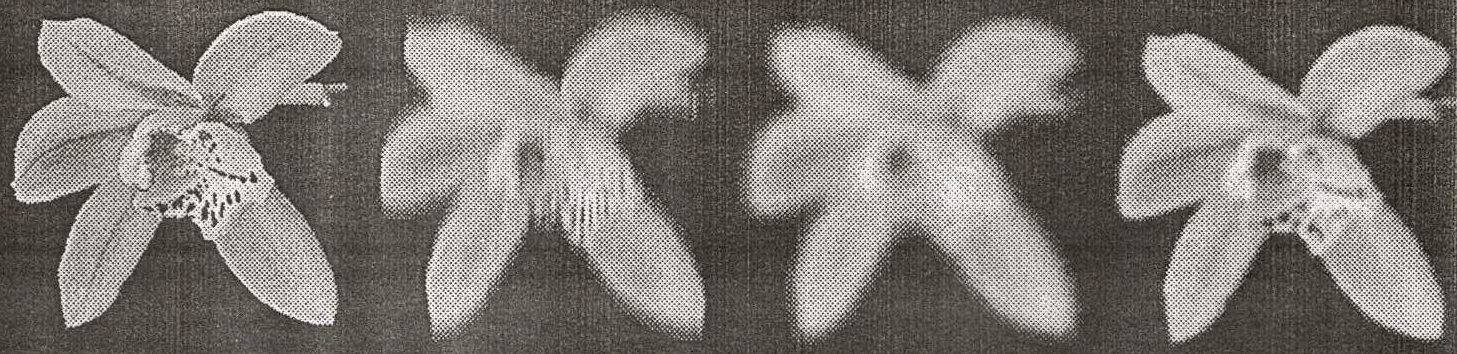
\includegraphics[width=12cm]{picture/png/screenshot001}

\hspace*{3.1cm}
\includegraphics[width=8.9cm]{picture/png/screenshot002}
\caption{Základní typy degradací. Nahoře zleva původní obrázek, obrázek rozmazaný pohybem, defokusací a turbulencí. Dole FT příslušné impulzní odezvy.}
\label{fig:screenshot001}
\end{figure}


\paragraph{a) Rozmazání pohybem} Je-li pohyb lineární (tj. po přímce) má impulsní odezva tvar obdélníka. 
\begin{itemize}
\item délka je úměrná délce expozice (při konstantní rychlosti pohybu)
\item šířka bude obrácená hodnota délky, abychom zachovali $\int h=1$ a nevnášeli tak do obrázku
jas. 
\item ve směru kolmém na směr pohybu se tento obdélníček chová jako $\delta$-funkce, tedy nic nemění. 
\end{itemize}

Po Fourierově transformaci obdržíme ve frekvenční oblasti známou funkci $\sinc(t) = \sin(t)/t$, natočenou do směru pohybu. 
Slangově se tato funkce označuje jako \emph{vlnitý plech}\footnote{Název zavedl J. Flusser :-)}. 

\begin{itemize}
\item nulové hodnoty funkce $H$ budou ležet na přímkách kolmých na směr pohybu. Čím blíže budou k sobě, tím je rozmazání 
větší. 
\item stejné nulové body budou zachovány i ve funkci $G$. Můžeme tak najít směr a délku pohybu (během
expozice). Získáváme odhad pro $H$ do Wienerova filtru. 
\end{itemize}

Podobně lze odhadovat impulsní odezvy na jiné druhy pohybu (např. dítě na houpačce). Některé druhy pohybů lze převést na
známé užitím souřadnicové transformace. Třeba rotační pohyb gramofonové desky při snímání shora, převedeme na pohyb 
lineární s konstatní (úhlovou) rychlostí pomocí radiálních souřadnic.

Při nekonstatních rychlostech je situace obtížná, protože se vytrácí polohová invariance.


\paragraph{b) špatné zaostření} Ideálním rozostřením světelného bodu je kruh. 
\begin{itemize}
\item ve skutečnosti klesá jeho intenzita ke krajům
\item impulsní odezva je tvaru válce -- přenosová funkce má nulové body na soustředných kružnicích
 \begin{align}
  H\sim \frac{J_1(r)}{r}\label{bessel}\qquad\begin{array}{ccl}\hbox{$J_1$}&\hbox{\dots}&\hbox{Besselova funkce 1. druhu}\\
  \hbox{$r$}&\hbox{\dots}&\hbox{radiální souřadnice}
  \end{array}
 \end{align}
Díky výrazu $\frac{1}{r}$ ve vztahu (\ref{bessel}) jsou Besselovy kmity tlumené.

\item stejné nulové body budou zachovány i ve funkci $G$. Postup je obdobný jako v případě lineárního posunutí.
Změříme vzdálenost kružnic, odhadneme impulsní odezvu a aplikujeme Wienerův filtr. 
\end{itemize}

\paragraph{c) turbulence} Vzniká např. při delší expoziční době, než je perioda Brownova pohybu částic v atmosféře. 
\begin{itemize}
\item impulní odezva (a přenosová funkce) jsou Gaussovy funkce. Nemají tedy nulové body a nelze proto použít metodu
z předchozích případů
\item k odhadu se používájí body, které nemění polohu, např. hvězdy ve snímcích oblohy (astronomie)
\end{itemize}

\subsubsection{Problém slepé dekonvoluce}
V obecném případě pro neznámé $h$ nemá úloha jednoznačné řešení. Zavádíme proto dodatečné omezující podmínky.

\begin{itemize}
\item nezápornost originálního signálu (snímku)
\item omezenost supportu $h$
\item minimalizace jistého potenciálového funkcionálu výsledného obrazu
\end{itemize}

Jiným problémem je tzv. \emph{vícekanálová slepá dekonvoluce}, kdy máme k dispozici několik stejných snímků s jinými
impulsními odezvami. Tedy systém
\begin{align}
g_1 &= f\conv h_1+n_1\\
&\vdots&\nonumber\\
g_l &= f\conv h_l+n_l
\end{align}

Tato úloha je nepoměrně snažší, protože máme daleko více informací a z každého $g_i$ jsme schopni zrekonstruhovat 
jiné části obrázku. Výsledek tedy můžeme \uv{poslepovat} z několika takových částí. Také jsme schopni daleko lépe 
odstraňovat případné šumy, podobně jako při průměrování více kopií.

\subsection{Geometrické zkreslení (geometrický inverzní problém)}
Model geometrického zkreslení obrazu lze zapsat jako
\begin{align}
g=T_G(f)
\end{align}

\subsubsection{Geometrická registrace (matching)}

Máme-li snímek téže scény z různých pohledů (tj. s jiným geometrickým zkreslením) a potřebujeme-li zjistit odpovídající
pixely (tj. aby stejné pixely měly stejné souřadnice), mluvíme o \emph{Registraci obrazu (image registration)}. Využití
spočívá např. v detekci časových změn. Nepřesná registrace vede na chybnou detekci resp. zjištění změn tam kde nejsou.

\paragraph{Kategorie registrace obrazu}
\begin{itemize}
	\item Different viewpoints -- multiview (vícepohledový)
	\item Different times -- multitemporal (vícečasový)
	\item Different modalities -- multimodal (multimodální)
	\item Scene to model registration
\end{itemize}

Registrace se provádí pomocí řídících bodů (control points). Pokud jsou správně nalezeny odpovídající řídící body v obou
obrazech, je možné sestavit geometrické transformace a snímky zregistrovat.

\paragraph{Postup registrace} se dá rozdělit do čtyř kroků:
\begin{enumerate}
	\item výběr kandidátů na řídící body,
	\item nalezení korespondence mezi kandidátskými body a výběr řídících bodů,
	\item odhadnutí modelu transformace souřadnic,
	\item vlastní transformace.
\end{enumerate}
Všechny kroky nejdříve stručně popíšeme a později se k ním vrátíme podrobněji.

\paragraph{Požadavky na řídící body}
\begin{itemize}
\item dobře automaticky detekovatelné
\item dostatečný počet
\item detekovatelné v obou obrazech
\item rozmístěny po celém snímku
\item invariantní k transformaci
\end{itemize}

Jako významné řídící body se volí \emph{rohy}, \emph{průsečíky} -- tyto jsou však citlivé na šum, \emph{těžiště uzavřených 
oblastí} -- na šum více stabilní, nebo \emph{extrémní křivosti křivek}.

V tomto prvním kroku se vybírají zvlášť na referenčním obrázku a zvlášť na registrovaném obrázku.

Po určení řídících bodů je třeba provést vzájemnou korespondenci. Tato operace se označuje jako (\emph{matching}). 
K tomuto účelu musíme mít dostatečně robusní, spolehlivou metodu, neboť některé body mohou chybět, mohlo dojít
k nepřesnostem atp. 

\paragraph{Matching}

Hledání odpovídajících bodů se provádí
\begin{itemize} 
\item topologicky (předpokládaný výskyt)
\item prohledává se okolí bodu s ohledem na intenzity (barvy) okolních pixelů
\end{itemize}

\vecobr{0.9}{contrpoint}{Postup při registraci dvou snímků}
\paragraph{Mapovací funkce (Mapping function design)}

Při vlastním mapování hledáme
\begin{align}
u &= f(x,y)\\
v &= g(x,y)\\
\noalign{\hbox{s podmínkou P1:}\nonumber}
u_i &= f(x_i,y_i)\\
v_i &= g(x_i,y_i)\qquad\forall i\in m,\ \hbox{kde $m$ je počet řídících bodů}
\end{align}
Funkce $f,g$ předpokládáme spojité a dost hladké, navíc parametrizovatelné (např. afinní transformace). 
Parametry funkcí hledáme řešením následujících úloh
\begin{itemize}
\item \emph{interpolační úloha} -- s podmínkou P1
\item \emph{extrapolační úloha} -- bez podmínky P1
\end{itemize}
Po nalezení funkcí již nic nebrání tomu, abychom obrazy namapovali bod po bodu.

\subsection{Výběr řídících bodů (control point selection) (matching) (?)}
Metody dělíme na \emph{signálově závislé} pracující s intenzitou obrázu a \emph{příznakové (signálově nezávislé)}.

\subsubsection{Signálově závislé metody}

\paragraph{Obrazová korelace} -- korelaci provádíme se skutečnými obrazovými hodnotami. Jeden obraz (okno)
posouváme po druhém a počítáme korelaci. Pokud existuje větší či menší shoda obrázku, bude na daném bodě ve výsledné matici
vysoká hodnota. Při konstatní korelační matici pak tento postup odpovídá počítání vztahu (?)
\begin{align}
\frac{\E\left[(X-\E X)(Y-\E Y)\right]}{\Var X \Var Y}
\end{align}
což odpovídá vztahu (?)
\begin{align}
C(X,Y)=\frac{\sum\limits_{i=0}^{N-1}
\sum\limits_{j=0}^{N-1}((X_{ij}-\bar{X})\cdot(Y_{ij}-\bar{Y}))}
{\sqrt{\sum\limits_{i=0}^{N-1}\sum\limits_{j=0}^{N-1}(X_{ij}-\bar{X})^2\cdot(Y_{ij}-\bar{Y})^2}}
\end{align}

Poznánmky k obrazové korelaci:
\begin{itemize}
	\item Metoda funguje dobře pro obrazy se stejnou intenzitou nebo pokud došlo ke globálním změnám kontrastu a jasu. Ostatní změny
dost vadí. V základním provedení by metoda fungovala jen pro posun. 

	\item Provádí se modifikace, kdy je korelační matice trojrozměrná. Časová náročnost je ale příliš velká, proto se metoda používá
pro malé rotace. Metoda dává dobré výsledky po hranové detekci v obou obrazech.

\item Urychlení výpočetní složitosti plyne z \emph{Korelačního teorému}
\begin{equation}
f\corr g \stackrel{\CFT}{\rightarrow}F\cdot G^\star
\end{equation}
kde symbol $(\cdot)^\star$ značí komplexně sdruženou matici

\item U této metody, se většinou nedetekují ŘB v druhém obrázku, ale hledají se nejvyšší korelace vzhledem k ŘB prvního obrázku. Nejčastěji hledáme malý výřez na velkém obrázku. Hodnoty intenzit se liší pouze lineárně.

\item V této podobě se metoda tolik nepoužívá, protože je výpočetně časově náročná a maximum bývá někdy „ploché“.

\item Proto modifikace: korelace hran, rohů, korelace ve frekvenční oblasti (fázová korelace), pyramidal representation (viz níže).

\end{itemize}

\paragraph{Fázová korelace} -- Fáze FT (když zahodíme amplitudy = spektrum se vydělí amplitudami) je blízká hranám obrázků. Ty jsou výhodnější kvůli nezávislosti na barvách a mají menší prostorovou korelaci. Nevracíme se hned do obrazové oblasti pro počítání korelace, ale zůstane se ve frekvenční, kde se využívá Fourier Shift Theorem (FST). Předpokládáme-li, že první a druhý obrázek jsou stejné, ale jen posunuté, máme dány funkce $f(\vec{x})$ a $g(\vec{x})=f(\vec{x} - \vec{a})$, kde $ \vec{x}, \vec{a} \in \mathbb{R}^2 $. Po Fourierově
transformaci bude
\begin{equation}
f(\vec{x})\stackrel{\CFT}{\longrightarrow} F(\vec{u})\qquad \quad \text{a} \qquad \quad g(\vec{x})\stackrel{\CFT}{\longrightarrow} e^{-2\pi i \vec{u} \cdot \vec{a} }F(\vec{u}),
\end{equation}
kde $ \vec{u} \cdot \vec{a} $ značí standardní skalární součin. Amplituda je u obou stejná, ale fáze se posunula o (?).

Definujeme tzv. Cross-power spektrum jako
\begin{equation}
\frac{F \cdot G^\star}{|F||G|}
\end{equation}
a protože se snažíme získat neznámý vektor posunutí $\vec{a}$, spočteme
\begin{equation}
\frac{F\cdot G^\star}{|F||G|} = \frac{F^2e^{2\pi i \vec{a} \cdot \vec{u}}}{|F|^2} \quad \stackrel{\ICFT}{\longrightarrow} \quad \delta(\vec{x}-\vec{a})
\end{equation}
Tím vznikne dobře lokalizovatelný pík. Metoda funguje dobře, odpovídá vlastně detekci hran a korelaci v obrazové oblasti.

\paragraph{nepodobnost (SSDA)} -- označuje se také jako \uv{klasická korelace}. Jde o použití jiné míry podobnosti než korelace. Ne $ L_2 $ norma, ale $ L_1 $ norma, např. $\sum|f_{ij}-g_{ij}|$. Hledá se bod, kde vztah $\sum|f_{ij}-g_{ij}|$ nabývá minima. Výpočet je velmi rychlý, protože suma neklesá, pouze roste -- jakmile jednou částečný součet převýší již vypočtené minimum, lze přímo přejít k dalšímu bodu.

Pro snadnou hardwarovou implementaci korelace jsou tyto metody (Fázová korelace a nepodobnost (SSDA)) dosti používané.

\paragraph{Rozšíření na obecnější transformace} rotace -- natáčení, okénko je kruh. Výpočetně velice náročné. Dá se nejdříve projet prostým posunutím, tam kde to zjistí maximum, tak to začnu natáčet. Vyberu úhel natočení, kde to je maximální. A poté projedu opět celý obrázek s tímto natočením.

\paragraph{Pyramidální reprezentace}
Snižujeme rozlišení obrázků o dvojnásobek -- začínám pak na nízkém rozlišení, kde najdeme „nadějné body“ a u vyššího rozlišení počítáme jen v okolí těchto bodů.


\subsubsection{Příznakové metody}

Jde o napočítávání vlastností -- \emph{příznaků} segmentovaných objektů obrazu. Příznaky by měly být invariantní k transformaci, kterou předpokládáme. Příznakem může být třeba \uv{plocha} objektu. Takový příznak je pak invariantní k posunu a rotaci, ale již nikoli k změně měřítka. Proto je třeba hledat příznaky sofistikovanější. Elementární množinu tvoří například příznaky vizuální (viz. dále) mezi které patří \emph{kompaktnost} = $ 4\pi \cdot \text{plocha} / \text{obvod}^2$, míra kompaktnosti, rektangularita a další. Složitější jsou pak příznaky diferenciální nebo momentové.

\subsubsection{???}

\paragraph{Point-based method} -- pro zjistění korespondence řídících bodů (matching) se vytváří úplný graf a hledají se 
4 parametry pro geometrickou transformaci (posun 2, rotace 1, měřítko 1). Porovnáváme po dvojici úseček a zjišťujeme,
jak ostatní body padají do okolí řídících bodů.

Další možnost je provést matching a zaznamenávat do parametrického prostoru provedenou transformaci. Pak hledat shluk
v tomto prostoru a vybrat tak nejlepší parametr.

Pro urychlení se nekonstruhuje úplný graf, ale třeba konvexní obálka nebo kostra grafu. Tím ovšem zavádíme do algoritmu výšší 
náchylnost k chybám a nestabilitě.

\vecobr{0.7}{match}{Zjištění vzájemné korespondence řídících bodů (matching)}

\paragraph{Region-based method} -- pro okolí řídících bodů hledáme společné charakteristiky, které by měli být
 \begin{itemize}
 \item \emph{invariantní vzhledem k transformaci} -- rotace, měřítko, \dots
 \item \emph{dostatečně diskriminabilní} \end{itemize}

\vecobr{0.7}{regbased}{Určování okolí bodů a jejich charakteristik (Region-based method)}

\paragraph{Kombinatorické (grafové)} Využívá globální informace o kandidátních bodech a jejich vzájemné polohy. Z níž hledá jejich korespondenci. Zkouší všechny možné kombinace a hledá tu nejlepší – jde o minimalizaci fce.

\paragraph{RST (rotation, scaling, translation)}
Libovolnou úsečku můžeme namapovat na libovolnou úsečku. V základním případě se každá dvojice bodů namapuje na každou dvojici z druhého obrázku. Tedy že namapujeme úsečku a podle ní transformujeme ostatní body a koukáme se, kolik bodů se shoduje se vzory – počítání zásahů. A pokud toto uděláme pro všechny dvojice bodů, můžeme pak říci, že ta transformace, která má nejvíce zásahů, je ta správná.

\subsection{Odhadnutí modelu transformace souřadnic}
Pro mapování chceme použít transformaci, která promítne řídící body prvního obrázku na odpovídající řídící body obrázku druhého. Transformační funkce má obecný tvar
\begin{equation}
x' = T_x (x) \qquad \qquad
y' = T_y (y)
\end{equation}
Tato transformace může platit pro celý obrázek (globální transformace), ale jednotlivé dílčí části můžou mít i odlišné transformace (lokální).

Většinou se transformace předpokládá jako jedna z následujících:
\paragraph{Affinní transformace}
\begin{equation}
x' = a_0+a_1x+a_2y \qquad \qquad
y' = b_0+b_1x+b_2y\label{afinita}
\end{equation}
Tato transformace
\begin{itemize}
\item zobrazuje čtverec na rovnoběžník,
\item zachovává přímky a jejich rovnoběžnost,
\item vyžaduje tři body pro její určení. V praxi se ale počítá z mnohem více bodů, pomocí metody nejmenších čtverců.
\end{itemize}
Affiní model je jeden z nejjednodušších, ale přesto se hojně používá
 
\paragraph{Perspektivní projekce}
\begin{equation}
x' = \frac{a_0+a_1x+a_2y}{1+c_1x+c_2y} \qquad \qquad
y' = \frac{b_0+b_1x+b_2y}{1+c_1x+c_2y}\label{perspekt}
\end{equation}

Perspektivní projekce je obecnější transformace. Má však tu vlastnost, že při pozorování z větších vzdáleností v afinitu
přechází, neboť $c_1$ a $c_2$ ve vztazích (\ref{perspekt}) budou malé.

\begin{itemize}
	\item V praxi se při transformacích ani projektivní nepoužívá, protože nevede na lineární soustavu a nejde ji nějak „rozumně“ řešit.
	\item Vystihuje promítání rovinných předmětů fotoaparátem.
	\item čtverec zobrazuje na jakýkoli čtyřúhelník
	\item nutné čtyři body
\end{itemize}

\vecobr{0.7}{trans}{Základní mapovací funkce}

\paragraph{Nelineární transformace}
\begin{equation}
x' = a_0+a_1x+a_2y+a_3xy\ [{}+a_4x^2+a_5y^2\ ] \qquad \qquad
y' = b_0+b_1x+b_2y+b_3xy\ [{}+b_4x^2+b_5y^2\ ]
\end{equation}
Tento model je silně nelineární, nezachovává přímky ani rovnoběžnost. Používá se často.

\subsubsection{K metodě nejmenších čtverců}
Předpkládejme parametrizovatelnou funkci $f(x,a_1,\dots,a_l)$ a k ní předem zadanou množinu bodů $U=\{[x_1,y_1],\dots,[x_K,y_K]\}$. Definujme funkci $d$ 
\begin{align}
d &= \sum\limits_{i=1}^K (f(x_i)-y_i)^2\label{minkvad}
\end{align}
Protože hledáme minumum funkce $d$, mluvíme o \emph{metodě nejmenších čtverců}. Položíme-li parciální derivace podle parametrů do rovnosti s nulou, dostáváme
\begin{align}
\frac{\partial d}{\partial a_i} &= 0\qquad\forall i\in \hat{K}
\end{align}
což je obecně nelineární systém rovnic, po jehož vyřešení a ověření, že se jedná o minimum, získáme námi hledané koeficienty. Vztah (\ref{minkvad}) lze obecně psát ve tvaru $\|U-f\|_\mathcal{N}$, kdy norma $\|\cdot\|_\mathcal{N}$ definuje nějakým způsobem vzdálenost bodů od hledané funkce (křivky).

\vecobr{0.9}{minkv}{K metodě nejmenších čtverců}

\subsection{Vlastní mapování (transformace)}
Vlastní mapování zabírá nejvíce výpočetního času. Musí se převzorkovávat, protože nové pixely mají neceločíselné souřadnice. Používají se přímé a nepřímé transformace.

\begin{itemize}
\item \emph{přímá (Forward)} -- procházíme všechny body ze zdrojového obrazu, transformujeme je a zapisujeme do výsledku. 
Vznikají situace, kdy se více bodů namapuje na stejné místo (přepisování) a výsledný obraz může obsahovat některé
prázné pixely (díry). Pro takové body je třeba provést interpolaci z okolních pixelů.

\item \emph{nepřímá (Backward)} -- procházíme všechny body výsledného obrazu a pomocí zpětné transformace určíme, který zdrojový bod
se na ně obrazí.
\end{itemize}

\paragraph{Lokální transformace}
Obrázek rozdělíme na trojúhelníky pomocí řídících bodů. Na každém trojúhelníku pak počítám affiní transformaci. Nemá spojité derivace a řeší se pomocí kubické transformace s 10 parametry, kde se předepíší spojitosti derivací.

Nejčastěji se používá TPS (Thin-Plate-Splines): hledá se minimální křivost plochy ideálně neformovatelného ocelového plátu fixovaného v řídících bodech.

Nelineární transformace se často provádí po trojúhelnících, na kterých se transformační funkce linearizuje 
(obdoba metody konečných prvků).
Pokud se použijí lineární polynomy, má tento postup za následek nepřirozené zalamování hran na přechodových stranách
trojúhelníkové sítě. Obecněji se proto definují \emph{Radiální bázové funkce}, které tyto vlastnosti nemají.
\begin{align}
u=\sum a_i\varphi_i(r_i)
\end{align}

\begin{figure}[htb]
\begin{minipage}[t]{0.33\textwidth}\captionsetup{width=0.9\textwidth}
\pngfigwithinfig{0.6}{lena}{Originální obraz}
\end{minipage}%
\hfill%
\begin{minipage}[t]{0.33\textwidth}\captionsetup{width=0.9\textwidth}
\pngfigwithinfig{0.6}{origspec}{Frekvenční spektrum originálu}
\end{minipage}%
\hfill%
\begin{minipage}[t]{0.33\textwidth}\captionsetup{width=0.9\textwidth}
\pngfigwithinfig{0.6}{lenaposkoz}{Obraz s periodickým poškozením}
\end{minipage}
\end{figure}

\begin{figure}[htb]
\begin{minipage}[t]{0.33\textwidth}\captionsetup{width=0.9\textwidth}
\pngfigwithinfig{0.6}{poskspec}{Frekvenční spektrum poškozeného obrazu}
\end{minipage}%
\hfill%
\begin{minipage}[t]{0.33\textwidth}\captionsetup{width=0.9\textwidth}
\pngfigwithinfig{0.6}{restorespec}{Upravené spektrum poškozeného obrazu}
\end{minipage}%
\hfill%
\begin{minipage}[t]{0.33\textwidth}\captionsetup{width=0.9\textwidth}
\pngfigwithinfig{0.6}{lenares}{Výsledný restaurovaný obraz}
\end{minipage}
\end{figure}

\section{Rozpoznávání dat (pattern recognition)}
\paragraph{Úloha rozpoznávání}
Máme $n$ tříd, máme rozhodnout o objektu $\mathcal{O}$ do jaké třídy patří.

Existují 2 přístupy: strukturární (syntaktické) a příznakové (statistické)
\begin{enumerate}
	\item strukturární
	\begin{itemize}
		\item založeno na teorii jazyků, rozhodování, zda patří slovo do jazyka
		\item příklad: dům, střecha, zdi, dveře, okna
	\end{itemize}
	\item příznakové
	\begin{itemize}
		\item příklad: žokejové $\times$ basketbalisté $\rightarrow$ příznaky: výška, váha
		\item pro každý objekt máme příznakový vektor (obecně tvořen čísly, vektory, maticemi, funkcemi atd.)
		\item nutné definovat metriku na prostoru příznaků (někdy problém)
	\end{itemize}
\end{enumerate}

\paragraph{Rozdělení na třídy}

Nabízí se například klasifikátor beroucí minimální vzdálenost od těžišť jednotlivých tříd.
\vecobr{0.7}{svestky}{Rozdělení na třídy}

\begin{itemize}
	\item Většinou máme k dispozici tzv. \emph{trénovací množinu} s daty.
	\item Otázka je podle jakého pravidla rozhodovat.
\end{itemize}
Příznakový prostor rozdělíme na oblasti (nadplochy), pak rozhodneme do které oblasti objekt padne.
\vecobr{1}{oblasti}{Rozdělení do oblastí}

Nejhorší případ je situace, kdy neznáme třídy (resp. počet), ani trénovací množinu. Pak v příznakovém prostoru
provádíme tzv. \emph{shlukování}.

\paragraph{Jak konstruhovat nadplochy?}

Pouhé zjišťování těžiště, nedává dobré výsledky. Lze také počítat rozptyly a podělit vzdáleností od těžišť.


Další algoritmus: vezmu dva body (o,x) a udělám dělicí přímku, pak testuji další body z trénovací množiny
a v případě špatné klasifikace posouvám, resp. natáčím přímku. (evidetně to lze udělat pouze pro lineárně separabilní
množinu).

Příklady klasifikátoru: minimální vzdálenost, minimální vzdálenost od těžišť, nejblišží soused (NN- nearest neighbour,
nebezpečné, citlivý na atypické prvky, není lineární klasifikátor)

\paragraph{NN -- Nearest neighbour}
\begin{itemize}
	\item modifikace: k-NN klasifikátor (přiřadíme do třídy, kde je $k$-nejbližších bodů) $\rightarrow$ $NN\equiv$ 1-$NN$
	\item k je třeba volit nízké oproti četnosti skupiny
\end{itemize}

Stále nerespektujeme rozložení četností $\rightarrow$ konstrukce statistických klasifikátorů.

\begin{tabular}{ccc}
	$\omega_1,\dots,\omega_n$ &\dots& individua\\
	$g_i(x)$ &\dots& rozhodovací funkce
\end{tabular}

Hledáme $\mathcal{G}=\max\limits_i g_i(x)$ (maximální ve smyslu nejlepší).

\subsection{Statistické klasifikace}

Náhodná veličina (NV) $\xi$, $E\xi$, $D\xi=E\left(\xi-E\xi\right)^2$.
\begin{align}
Cov(\xi,\nu) &= E(\xi-E\xi)(\nu-E\nu)\\
Cor(\xi,\nu) &= \frac{Cov(\xi,\nu)}{\sqrt{D\xi D\nu}}
\end{align}

\paragraph{Bayesův klasifikátor}

\begin{equation}
p(\omega_i|x)=\frac{p(x|\omega_i)p(\omega_i)}{\sum\limits_j p(x|\omega_j)p(\omega_j)}
\end{equation}

\begin{description}
	\item[$p(\omega_i|x)$] \dots pravděpodobnost, že individum bude patřit do $i$-té třídy, přičemž 
	jsme na něm naměřili příznakový vektor $x$
	\item[$p(\omega_i)$] \dots pravděpodobnost $i$-té třídy v $\Omega$
	\item[$p(x|\omega_i)$] \dots pravděpodobnost, že na prvku ze třídy $i$ můžeme naměřit vektor $x$
\end{description}

Pravděpodobnosti $p(\omega_i)$ určíme buď z relativních četností trénovací množiny, v tom případě je nutné
zajistit, aby četnosti odpovídaly skutečnosti, nebo předpokládáme pro všechny třídy \emph{stejnou} pravděpodobnost
tj. $p(\omega_i)=\frac{1}{n},\ \forall i\in \hat{n}$, kde $n$ je počet tříd.

Nyní je třeba určit $p(x|\omega_i)$ pro každou třídu. Předpokládejme rozložení $x$ ve třídě jako normální. Pomocí
trénovací množiny odhadneme parametry tohoto rozložení. Pro jednorozměrný příznakový vektor máme
\begin{equation}
p(x) = \frac{1}{\sigma \sqrt{2\pi}}e^{-\frac{(x-\mu)^2}{2\sigma^2}}
\end{equation}
Pro vícerozměrný příznakový vektor pak
\begin{equation}
p_N(\bm x) = \frac{1}{(2\pi)^\frac{N}{2}\sqrt{|\bm \Sigma|}}e^{-\frac{1}{2}(\bm x-\bm m)^T\bm \Sigma^{-1}(\bm x-\bm m)}
\end{equation}

kde $\bm \Sigma_{ij}=Cov(\xi_i,\nu_j)$ tj. kovariance $i$-tého a $j$-tého příznaku.

\paragraph{Příklad:}
Pro $N=2$ bude
$$
\Sigma=\left(\begin{array}{cc}\sigma_1^2 & Cov\\ Cov & \sigma_2^2\end{array}\right)
$$

Je-li $Cov=0$ vytvoří případ $\sigma_1=\sigma_2$ kružnici, $\sigma_1\neq\sigma_2$ elipsu v základní poloze.
Kovariance nenulová pak vede na elipsu v obecné poloze.

Každá třída má tedy vlastní Gaussovu funkci s vlastní kovarianční maticí $\Sigma$.
Pokud budou pouze dvě třídy a $\Sigma_1=\Sigma_2$, případ odpovídá Euklidovskému určování vzdáleností.

\paragraph{Pozn.} Výraz $(\bm x-\bm m)^T\Sigma(\bm x-\bm m)$ definuje tzv. Mahalanobisovu vzdálenost.\\
Rovnost kovariančních matic je ekvivalentní skutečnosti, že je Bayesův klasifikátor \emph{lineární}.\\
Pokud jsou tedy kovariančních matic stejné a změní se apriorní rozdělení 
pravděpodobností $(p(\omega_i))$, posunuje se rozdělovací přímka od množiny s větší pravděpodobností.

\vecobr{0.7}{bayes}{Posun rozdělovací přímky lineárního Bayesova klasifikátoru při změnách $p(\omega_i)$. Vpravo
	extrémní případ nulové četnosti.}

Testování klasifikátoru, provádíme tak, že množinu předem klasifikovaných dat rozdělíme jednak na trénovací a
testovací. Parametry určíme z trénovací množiny.

\paragraph{Možné chyby}
\begin{itemize}
	\item chyba modelu (není to např. normální rozložení)
	\item rozložení (byť normální) nemusí mít stejné parametry, někdy lepší 3 třídy klasifikovat jako dvě a pak tu
	jednu následně rozdělit
	\item chyby v odhadech kovarianční matice (celkem $\approx\frac{n^2}{2}$ prvků), pokud máme málo dat, 
	použijeme předpoklad o stejných kovariančních maticích, pak na odhady lze použít data všech tříd.
	\item chyba předpokladu diagonální matice (příznaky jsou většinou silně korelované)
	\item curse of dimensionality (prokletí dimenze) -- moc příznaku $\Rightarrow$ stejná testovací data $\Rightarrow$ 
	více parametrů $\Rightarrow$ chyby $\Rightarrow$ Je potřeba aspon $10\times$ více prvků než příznaků.
\end{itemize}

\paragraph{Odhady parametrů}

Maximum likelihood test:
\begin{equation}
\max\limits_q\prod\limits_{k=1}^N p(x_k|q)
\end{equation}

$k$ $\dots$ index v trénovací množině. Uděláme logaritmus a vyšetříme extrém funkce tj. ($\frac{\partial}{\partial q}=0$).
Což vede na lineární rovnice a odhady parametrů
\begin{align}
e &= \frac{\sum x_i}{N}\\
\sigma^2 &= \frac{1}{N}\sum(x_i-e)^2
\end{align}

V předchozím jsme předpokládali parametrické odhady.

\paragraph{Neparametrické odhady} používáme až selžou parametrické odhady.

\begin{itemize}
	\item hustotu pravděpodobnosti na intervalech odhadneme pomocí relativních četností realizací
	\item vylepšení -- odhad po bodech (posouváme interval po bodech)
	\item nejlepší určení spojité hustoty pravděpodobnosti -- metoda Parzenova okna
\end{itemize}

Provádíme průměrování relativních četností nějakou váhovou funkcí, aby centrální bod měl větší váhu, 
možné použít Gaussovu funkci. Dost záleží na tom, jak zvolíme šířku okna (support funkce) $w$. Extrémem 
jsou:
\begin{itemize}
	\item $w=1$ $\dots$ Dirackova $\delta$-funkce, dostáváme jednotlivé realizace s pravděpodobností $\frac{1}{n}$
	\item $w=\max$ $\dots$ dostaneme konstatní hustotu po celém intervalu. 
\end{itemize}

Malá okna vedou na přetrénování neboli \emph{overtraining} -- na trénovací množině to funguje bezchybně, ale na ostatních
datech nespolehlivě.

\vecobr{0.8}{cetnosti}{Určování četností}

Pokud klasifikace stále selhává a vše je již optimalizované, nezbývá než zkusit změnit trénovací množinu nebo
brát jiné příznaky. Často se používájí kombinace více klasifikátorů $\mathcal{K}_1,\dots,\mathcal{K}_L$, protože 
některé fungují jen na určité příznaky. Pokud $k$-klasifikátor určí $p_k(\omega_i|x)$ bereme jako kombinovaný
klasifikátor $\mathcal{K}$ jednu z těchto možností:
\begin{align}
p(\omega_i|x) &= \max\limits_i\prod\limits_{k=1}^L p_k(\omega_i|x)\\
p(\omega_i|x) &= \max\limits_i \sum\limits_{k=1}^L p_k(\omega_i|x)\\
p(\omega_i|x) &= \max\limits_i \max\limits_{k\in\hat{L}} p_k(\omega_i|x)
\end{align}

\subsection{Klasifikace bez učení (shluková analýza)}

Shlukovou analýzu neboli \emph{clustering} používáme, když předem neznáme počet tříd. Shluk není přesně definován,
ale znamená zhruba to, že rozptyly parametrů ve shluku jsou \uv{malé}, naproti tomu vzdálenosti jednotlivých shluků
\uv{velké}. 

V obecné definici můžeme shluk považovat za libovolnou podmnožinu dat, a tedy proces shlukování pak lze přirovnat k pokrytí
celé množiny disjunktními podmnožinami.

Míru kvality shluků lze určit jako

\begin{equation}
Q=\sum\limits_{i=1}^N\sum\limits_{x\in C_i}\|x-m_{C_i}\|^2
\end{equation}

Pokud známe počet shluků, metoda funguje dobře, pokud ne, snaží se udělat z každého prvku samostatný shluk.

\paragraph{$N$-means clustering algoritmus}
\begin{enumerate}
	\item vyberem $N$ středních hodnot ($\times$)
	\item klasifikujeme všechny objekty minimální vzdáleností $\rightarrow$ dostáváme shluky
	\item přepočítáme těžiště
	\item opakujeme postup pokud těžiště mění své polohy 
\end{enumerate}

Často dává dobré výsledky, ovšem je zde silná závislost na počátečních podmínkách.
\vecobr{0.7}{clustering}{Ukázka shlukování a závislost procesu na počátečních podmínkách.}

\paragraph{Jiné přístupy}

\begin{itemize}
	\item Data bereme jako jeden počáteční shluk a pro pevný bod zkoumáme, jak se změní kritérium kdybychom
	objekt přesunuli k tomuto shluku. Pokud se zmenší, přepočítáme těžiště a postup opakujeme.
	\item \emph{Algoritmus ISODATA} Nejdříve máme tolik shluků jako je objektů a shluky spojujeme. Nebo máme počáteční shluk,
	který postupně rozdělujeme. Při tom se využívá konstrukce tzv. \emph{dendrogramu}.
	\item Podmínky pro zastavení jsou např. počet shluků nebo rozptyl největšího shluku.
\end{itemize}

\paragraph{Kriteria pro spojení shluků}
\begin{align}
f &= \min\limits_{a,b}\rho(a,b)\\
f &= \max\limits_{a,b}\rho(a,b)\\
f &= \rho(\mu_i,\mu_j)\\
\noalign{\hbox{\emph{Hausdorfova metrika: }}}\nonumber
f &= \max(\max\limits_a\rho(a,B),\max\limits_b\rho(b,A))
\end{align}

Hausdorfova metrika je dosti náročná na výpočet. Je jasné, že shlukovací proces na zvolené metrice silně závisí.

Pokud nemáme počet shluků, je úloha obtížná, potom rozdělujeme jeden shluk na malé shluky a počítáme hodnotu
kritéria $J_i$. Pak vynášíme graf $J_i$ pro $i$ rovno $1,2,\dots,N$ shluků a optimální počet shluků je pak $N_0$
takové, kde derivace křivky začne růst o poznání pomaleji \refobr{shluky}.

\vecobr{0.7}{shluky}{Ukázka vynášení globálního kritéria pro spočítané shluky a předpokládané optimální shlukování.}

{\def\mez{\hskip0em}
	\def\scal{0.35}
	\def\mezv{\vskip12pt}
	\begin{figure*}[htb]%
		\centerline{%
			\begin{tabular}{c}\scalebox{\scal}{\includepng{vys000_.ppm}}\\$iter= 0$\end{tabular}\mez%
			\begin{tabular}{c}\scalebox{\scal}{\includepng{vys001_.ppm}}\\$iter= 1$\end{tabular}\mez%
			\begin{tabular}{c}\scalebox{\scal}{\includepng{vys002_.ppm}}\\$iter= 2$\end{tabular}\mez%
			\begin{tabular}{c}\scalebox{\scal}{\includepng{vys003_.ppm}}\\$iter= 3$\end{tabular}\mez%
		}
		\mezv
		\centerline{%
			\begin{tabular}{c}\scalebox{\scal}{\includepng{vys004_.ppm}}\\$iter= 4$\end{tabular}\mez%
			\begin{tabular}{c}\scalebox{\scal}{\includepng{vys005_.ppm}}\\$iter= 5$\end{tabular}\mez%
			\begin{tabular}{c}\scalebox{\scal}{\includepng{vys006_.ppm}}\\$iter= 6$\end{tabular}\mez%
			\begin{tabular}{c}\scalebox{\scal}{\includepng{vys007_.ppm}}\\$iter= 7$\end{tabular}\mez%
		}\mezv%
		\centerline{%
			\begin{tabular}{c}\scalebox{\scal}{\includepng{vys008_.ppm}}\\$iter= 8$\end{tabular}\mez%
			\begin{tabular}{c}\scalebox{\scal}{\includepng{vys009_.ppm}}\\$iter= 9$\end{tabular}\mez%
			\begin{tabular}{c}\scalebox{\scal}{\includepng{vys010_.ppm}}\\$iter= 10$\end{tabular}\mez%
			\begin{tabular}{c}\scalebox{\scal}{\includepng{vys011_.ppm}}\\$iter= 11$\end{tabular}\mez%
		}%
		\caption{Ukázka shlukovaní ve 2D metodou matematické morfologie.}
		\label{shlukpic}%
	\end{figure*}%
}

\vecobr{0.6}{shlukygraf}{Graf závislosti počtu shluků na počtu iterací. Za optimální by se dala považovat druhá iterace
	s dvanácti shluky.}


\subsection{Redukce dimenzionality (příznakového prostoru)}
Z naměřených dat máme většinou obrovské množství příznaků, ty jsou však silně korelované, proto se prostor 
snažíme redukovat.

\begin{itemize}
	\item \emph{One-class problem} -- cílem je vybrat optimální reprezentaci (tj. $x$ příznaků), které charakterizují 
	všechny objekty celé množiny
	\item \emph{Two-class problem} -- cílem je najít $y<x$ příznaků, aby se jen velmi málo ztratila informace
\end{itemize}

\paragraph{Přístupy:}
\begin{enumerate}
	\item Feature selection -- vybíráme nějaké příznaky (používá se pro Two-class)
	\item Feature extraction -- hledáme zobrazení do méně rozměrného prostoru (používá se pro One-class)
\end{enumerate}

\paragraph{One-class}

Hlavní myšlenka vychází z toho, že korelované příznaky vytváří v příznakovém prostoru (PP) více či méně protáhlou
elipsu v níž můžeme kratší poloosu považovat za šum a za příznaky brát souřadnice průmětů bodů z PP do hlavní poloosy
této elipsy.
\refobr{oneclass}.
\vecobr{0.8}{oneclass}{Ukázka redukce dimenzionality korelovaných příznaků}

\paragraph{Principle component transformation -- PCT (Karhunen, Loeve)}
Tato transformace používá rotaci a hledá nejlepší úhel pro nekorelovanost. 
Je založena na transformaci SVD. Nekorelovaná matice (tedy ta, kterou hledáme) bude diagonální. Můžeme použít postup:

\begin{enumerate}
	\item $K_x$ $\dots$ matice korelace, pokud je diagonální, končím.
	\item Provedeme SVD tj. $K_y=GK_xG^T$. Získáme $K_y$, která je diagonální. Příznaky jsou pak $y=Gx$.
\end{enumerate}

Protože $K_x$ je původně symetrická, lze diagonalizaci provést a matici transformace dokonce volit ortonormálně.
Nalezená vlastní čísla pak jsou zároveň rozptyly; matici $G$ sestavíme z přidružených vlastních vektorů.

Předchozí myšlenka, že malé rozptyly znamenají šum ale nefunguje pro \emph{two-class}. Právě na základě jich
jsme schopni třídy rozlišit \refobr{twoclass}.
\vecobr{0.8}{twoclass}{Two-class problém a nemožnost zanedbat příznaky s malým rozptylem, neboť hrozí ztráta rozlišovací
	schopnosti}

\paragraph{Two-class a feature selection}

Dobře rozdělené třídy, uvažujeme-li jeden příznak, budou mít vysokou hodnotu funkce $\Phi$
\begin{equation}
\Phi=\frac{(\mu_1-\mu_2)^2}{(\sigma_1^2+\sigma_2^2)}
\end{equation}

Výraz $(\mu_1-\mu_2)^2$ se nazývá \emph{interclass deviation}. Je vidět, že čím je větší, tím lépe jsou třídy odděleny.
Ve vektorovém pojetí $(\sum((\bm \mu_1-\bm \mu_2)_i)^2)$ tato funkce funguje dobře za předpokladu, že jsou příznaky nekorelované (to bohužel v praxi 
není příliš často). 

Předchozí operace byly provedeny na trénovacích množinách, tím vznikly parametry pro třídy $\bm m_1, \dots, \bm m_K,
\Sigma_1,\dots,\Sigma_K$, kde $K$ je počet tříd. Mezi dvěma třídami tak můžeme definovat známou \emph{Mahalanobisovu 
	vzdálenost} pro třídy v příznakovém prostoru:
\begin{align}
d_M=(\bm m_1-\bm m_2)(\Sigma_1+\Sigma_2)^{-1}(\bm m_1-\bm m_2)^T\\
\noalign{\hbox{Reps. vylepšení od \emph{Bhattacharge}}}\\
d_B=\frac{1}{4}d_M+\frac{1}{2}\ln\frac{|\frac{1}{2}(\Sigma_1+\Sigma_2)|}{\sqrt{|\Sigma_1||\Sigma_2|}}
\end{align}

Pokud chceme pouze vybrat příznaky (tj. $D$ příznaků a chceme z nich vybrat $d$, tak aby $d<<D$), vyčíslujeme
$d_M$ (resp. $d_B$) a hledáme $d$-tici, kdy $d_M$ (resp.$d_B$) bude maximální.

\paragraph{Algoritmus Branch \& Bound}
Myšlenkou algoritmu je efektivní procházení celého stromu příznaků (viz obr. \ref{branchandbound}). Strom má ve 
svých uzlech $k$-tice příznaků. Strom se odvíjí od kořene, kde je celká $D$-tice příznaků, k listům, ve kterých už je jen
$d$-tice příznaků. V každém následujícím patře stromu ubyde jeden příznak. Strom procházíme od kořene k listům
a v každém uzlu spočteme kritérium ($K=d_M(\langle k$-tice$\rangle)$. Hodnota $K$ se zanořováním hlouběji do stromu bude zmenšovat, až
dojdeme k prvnímu listu. Zde si uložíme $V=K$ a jdeme k dalším uzlům. Nyní po výpočtu $K$ testujeme zda $K>V$. Pokud
to neplatí (tj. $K\leq V$), můžeme zahodit celý podstrom, protože hodnota $K$ se bude dál jen snižovat a my se 
přece snažíme najít $d$-tici pro které je $K$ maximální. Pokud se dostaneme opět do listu a je $K>V$, 
aktualizujeme hodnotu $V$ na $K$ a zapamatujeme si tento list. Tak postupujeme dále až projdeme celý strom.


\vecobr{0.7}{branchandbound}{Algoritmus Branch \& Bound při výběru 2 ze šesti příznaků.}


\subsection{Suboptimální metody}
Protože \emph{fullsearch} příznaků je značně pomalý, provádí se místo něj následující heuristické algoritmy.

\paragraph{Algoritmus Sequentional forward selection (SFS)}
\begin{enumerate}
	\item vyberu nejlepší příznak
	\item přidám příznak, který vyváří nejlepší dvojici s předchozím
	\item[$\vdots$]
	\item v $k$-tém kroku přidám příznak, který s předchozí $(k-1)$-ticí vytváří nejlepší $k$-tici vzhledem ke kritériu.
\end{enumerate}

V základním provedení má vady, protože nelze vyhodit příznak a přidáváme pouze po jednom. Takže vylepšení:
přidávat $j$-tice (v rámci $j$-tice to je \emph{fullsearch}). Algoritmus lze samozřejmě modifikovat 
místo procesu \emph{forward} na odebírání tj. \emph{backward}.

\paragraph{Algoritmus Plus $l$ minus $s$}
Tento je opět rozšířením originálního SFS algoritmu. V daném kroku lze přidat $l$-tici a odebrat $s$-tici příznaků.
V rozšířené verzi navíc $l$ a $s$ jsou dynamické. Algoritmus údajně velice dobře funguje. 

\section{Rozpoznávání v obraze}
\subsection{Segmentace}
Patří sem:
\begin{itemize}
	\item hledání objektů v obraze
	\item oddělení objektů od pozadí
	\item je třeba uchovat informace, kde se objekt nachází
\end{itemize}

Základní tři metody pro segmentaci obrazu:
\begin{enumerate}
	\item Prahování (Thresholding)
	\item Spojování hran (Edge linking)
	\item Růst oblasti (Region growing)
\end{enumerate}

\paragraph{ad 1) Prahování}
Histogram objektu je tzv. bimodální -- má 2 lokální maxima -- jedno odpovídá objektu jedno pozadí. Nalezneme lokální minimum mezi nimi -- práh. To co je pod prahem položíme rovno 0 a to co je nad prahem položíme rovno 1. Tím vznikne binární obrázek. Ideální je použití na (skoro) binárních obrázcích \refobr{hist}.
\begin{itemize}
	\item Lze provést i jen lokální prahování.
	\item Teoreticky možné použít i více prahů.
\end{itemize}

\vecobr{0.8}{hist}{Histogram obrázku a zvolený práh pro segmentaci typu popředí/pozadí}

\paragraph{ad 2) Spojování hran}

\emph{Hrana} je informace v obrazové oblasti. \emph{Hranice} pak je informace vyšší úrovně, měla by být souvislá, 
jednobodová.

Určení hranic se většinou provádí následujícím postupem.

\begin{enumerate}
	\item hranový detektor
	\item binarizace prahováním s vysokým prahem -- zůstane jen vysoký gradient
	\item zbavení se \emph{izolovaných bodů} -- pomocí morfologických operací
	\item zmenšení tloušťky na jeden pixel
	\item napojování částí
\end{enumerate}

Při napojování částí se prohledává okolí $A$ koncového bodu jedné hranice a podle určitého kritéria se rozhoduje, zda sousední hranice v $A$ napojit nebo ne. Další možností je použít hranové detektory založené na funkcionálech, ty často vytvářejí automaticky uzavřené křivky.

Díky špatným výsledkům se to moc nepoužívá (?).

\vecobr{0.8}{napojeni}{Prohledávání okolí a napojování hranice}

\paragraph{ad 3) Růst oblastí}
Je potřeba specifikovat tzv. semínka (\emph{seed points}), od nich se pak provádí buď numerická simulace roztahování
křivky v závislosti na gradientu obrázku a křivosti nebo jisté prohledávání okolí a následný růst křivky do něj.
Semínka buď určuje uživatel nebo se provede hrubá hranová detekce s velkým prahem a semínko se zvolí mimo hranu.
\vecobr{0.8}{growing}{Region growing s počátečními body (semínky)}

Prohledává se okolí zárodečného bodu -- testuje se kritérium homogenity (nejjednodušší způsob je testování úrovně šedi)
\begin{itemize}
	\item pokud je kritérium splněno, přidám bod do oblasti a pokračuji s jeho okolímˇ
	\item možné odlišnosti:
\begin{itemize}
	\item kritérium homogenity -- úroveň jasu nebo barev, textura
	\item způsob prohledávání okolí bodů
\end{itemize}
\end{itemize}
V současnosti:
\begin{itemize}
	\item funkcionál, v jehož minimu je fce, která aproximuje původní jasovou fci funkcí po částech konstantní
	\item minimalizační úloha
\end{itemize}

Někdy je výhodné objekt reprezentovat pomocí kvadraturového stromu, protože ten vytváří
homogenní oblasti. Ty se pak můžeme snažit spojovat.
\vecobr{0.7}{kvadtree}{Vytvoření kvadraturového stromu a spojení oblastí do hranice}

\paragraph{Popis hranice}
Uvažujeme-li nyní binární obrázek a v něm křivku, můžeme k její reprezentaci využít tzv. \emph{chain codes} tedy
řetězce čísel, kde následující číslo popisuje směr bodu oproti stávajícímu. Pokud definujeme 4 (absolutní) směry
(0 -- nahoru, 1 -- doleva, 2 -- doprava, 3 -- dolů), lze křivku zapsat jako např. 020233231110. Při použití 
relativního vyjádření stačí 3 hodnoty (0 -- rovně, 1 -- doleva, 2 -- doprava). Procházíme křivku a zapisujeme
0 pokud neměníme směr, 1 resp. 2 když křivka zatáčí. Svislé a vodorovné části se pak vyobrazí jako sekvence nul.

\paragraph{Problém hranice}
V diskrétním rastru vzniká problém, zda za hraniční pixely považovat ty, které sdílí stěnu nebo zda stačí, sdílí-li 
společný bod. Následkem toho můžeme definovat čtyřokolí a osmiokolí bodu a tím i čtyř-spojitost (resp. osmi-spojitost).

\vecobr{0.7}{okoli}{Ukázka nejednoznačnosti hranice. Definice 4-okolí, 8-okolí}
\vecobr{0.8}{diler}{Dilatace a eroze objektu s kruhovým objektem}

\subsection{Matematická morfologie}
Máme-li v obraze objekty s velmi členitou hranicí jde jistými operacemi tyto \uv{záhyby} zahladit.

\paragraph{Morfologické operace}
Předpokládejme v obraze dva objekty $A,B$ reprezentované nějakým způsobem v obraze. Definujeme operace:
\begin{description}
	\item[Dilatace $\oplus$ (expanze):] $A\oplus B=\{x|B_x\cap A\neq \emptyset\}$
	\item[Eroze $\ominus$:] $A\ominus B=\{x|B_x\subset A\}$
\end{description}

Za objekt $B$ volíme vetšinou malý kruh, takže dilatace odpovídá objíždění $B$ po hranici $A$ a zahlazování zálivů.
Objekt se mírně rozšiřuje. Eroze odpovídá objíždění hranice $A$ z vnitřní strany a zahlazování výběžků. Výsledný objekt
se zmenšuje \refobr{diler}.
Bude-li objekt $B$ symetrický, pak z množinových operací vyjde vztah

\begin{equation}
(A\ominus B)^C=A^C\oplus B\quad\hbox{kde operace $(\cdot)^C$ značí doplněk množiny}
\end{equation}

Tak můžeme definovat operace \emph{otevření} a \emph{uzavření} objektu:
\begin{description}
	\item[Otevření:] $A\circ B=(A\ominus B)\oplus B$\quad$\rightarrow$ vyčistí výběžky
	\item[Uzavření:] $A\bullet B=(A\oplus B)\ominus B$\quad$\rightarrow$ vyčistí zálivy
\end{description}

\paragraph{Požadavky na příznaky:}
\begin{description}
	\item[1. Invariance] -- Objekty uvnitř třídy musí mít podobné vlastnosti.
	\item[2. Diskriminabilita] -- Příznaky musí být s to rozlišit příslušnost k dané třídě.
	\item[3. Stabilita (robustnost)] -- Je potřeba, aby příznaky rozumně reagovaly na případný šum. Stejně tak malá odlišnost
	objektu by se měla odrazit v malé změně hodnoty příznaku.
	\item[4. Efektivita] -- Nenáročnost na výpočet příznaku, pokud možno menší počet příznaků.
\end{description}

\def\R{\mathbf{R}}
Předpokládejme příznakový prostor $\mathcal{P}$ a metriku $\rho$, dále $G$ souvislou, omezenou oblast v $\R^2$

Příznaky můžeme rozdělit na:
\begin{description}
	\item[1. Intuitivní (visual features)] -- barva, plocha, obvod, \dots
	\item[2. Transformační] -- jako příznaky se berou koeficienty potřebné k dané transformaci
	\item[3. Momenty ] -- převod objektu do polynomiální báze $\mathcal{X}=\{x^py^q\}$
	\item[4. Diferenciální] -- například části hranice aproximované hladkou křivkou
\end{description}

\subsection{Intuitivní příznaky}
\begin{itemize}
	\item obsah (P), obvod (o) -- Tyto příznaky nejsou invariantní na změnu měřítka,
	navíc spousta úplně odlišných objektů může mít stejný obsah resp. obvod.
	\item minimální opsaný obdélník (poměr jeho stran)
	\item Kompaktnost -- $C:=\frac{4\pi P}{o^2}$, pro jednotkový kruh vyjde 1
	\item Míra konvexnosti -- tj. poměr obsahu objektu $P$ a obsahu jeho konvexního obalu $P^\prime$. ($\frac{P}{P^\prime}$)
	\item Eulerovo číslo -- tj. počet kompoment $C$ minus počet děr $H$. ($C-H$)
\end{itemize}
Výše uvedené příznaky se používají k předtřídění při velkém množství tříd. Obecnou nevýhodou je slabá diskriminabilita,
výhodou naopak rychlé napočítání

\paragraph{Jak zajistit invarianty vzhledem k translaci?} -- stačí funkce přepočítávat s ohledem na těžiště.

\subsection{Transformační příznaky}
Chceme-li charakterizovat nějakým způsobem objekt, lze použít tzv. \emph{shape-vector}, což je posloupnost vzdáleností
od těžiště objektu k jeho okraji po jistých úhlových přírustcích. 

Složky Shape-vectoru $(a_k)$ nejsou primárně invariantní na rotaci objektu ani na změnu měřítka. Pokud chceme 
zajistit invarianci na změnu měřítka, vybereme maximální vzdálenost, od ní začneme a složky podělíme touto maximální
vzdáleností. Problém vzniká, pokud je takových složek více, resp. když je spousta složek blízkých této vzdálenosti.

\vecobr{0.8}{shapevec}{Konstrukce Shape-vectoru}
Invarianci na rotaci přímo nezajistíme, museli bychom rotovat posloupnost. To ovšem můžeme nahradit operací
korelace. Která nám nalezení shody zajistí.

Druhý způsob je obejít všechny možné rotace trikem.
Pokud provedeme $FFT$, dostaneme komplexní vektor $(A_k)$. Z FFT shift-teorému plyne, že můžeme porovnávat 
absolutní hodnoty složek tohoto vektoru. Ty totiž budou invariantem, neboť počáteční posun (v tomto případě počáteční úhel,
od kterého tvoříme shape-vector) se po $FFT$ převede na komplexní jednotku, která násobí původní funkci, takže v absolutní
hodnotě se vektor nezmění. Dva Shape-vectory budou po složkách splňovat vztah
\begin{align}
{A'}_k &= e^{-i\pi\varphi}A_k\\
\noalign{\hbox{tedy}\nonumber}\\
|{A'}_k| &= |e^{-i\pi\varphi}||A_k|=|A_k|=\sqrt{\Re^2A_k+\Im^2A_k}
\end{align}

Shape-vektory dobře fungují jen na tzv. \emph{hvězdicovité objekty}. Objekty ale bývají složitější. Proto vezmeme
kružnicovitou síť, začneme opět od maximálního bodu a pokud objekt překrývá více než polovinu segmentu, zapisujeme
do tzv. \emph{tvarové matice} 1 jinak 0 \refobr{krsit}. 
\begin{itemize}
	\item[$+$] každý objekt má stejně velkou matici, stejným počtem mezikruží zajistíme i invarianci na změnu měřítka
	\item[$-$] velké paměťové nároky
	\item[$-$] stejná míra váhy pro velké i malé segmenty $\rightarrow$ poloměry se volí, aby segmenty měly stejnou plochu
\end{itemize}
Metoda údajně velmi dobře funguje.
\vecobr{0.8}{krsit}{Příznaky tvořené mezikruhovými segmenty}

\paragraph{Rozpoznávání polozakrytých objektů}
Výše uvedené příklady nefungují, protože zakrytí změní celý vektor. Tvarová matice také nelze použít, protože se
podstatně změnilo těžiště. U binárních objektů lze vzít lokální vlastnosti hranice -- diferenciální invariance.

Definuje se metrika jakožto délka shody s hranicí v databázi. To je sice dobré, ale je potřeba hranici zapsat i s 
derivacemi vyšších řádů, tím je to zase náchylné na šum, což opět vede na malou použitelnost v praxi.

Dalším nápadem je třeba rozsekat objekt na menší objekty a počítat klasické příznaky a ty pak v rámci objektu globálně 
sloučit. Tato metoda funguje dobře na polygonech, takže nejdříve je potřeba objekt \emph{aproximovat polygonem}, což
někdy bývá obtížné. Při porovnání dvou objektů musíme totiž udělat i stejné dělení.

Pro hladkou křivku můžeme za příznaky brát \emph{inflexní body (IB)} tj. řešení rovnice $\ddot{x}\dot{y}-\ddot{y}\dot{x}=0$.
Tyto invarianty se chovají dobře při afinní transformaci. Pro představu stačí vzít počet inflexních bodů.
Problém vzniká při napočítávání. Hodnoty bývají blízké nule, takže je třeba vhodně volit práh. Objekt rozdělíme podle 
inflexních bodů, ty následně spojíme a bereme \uv{odřezky} pro opakování postupu. Hledání IB je nestabilní.

Lepší a spolehlivější metody zatím nebyly objeveny.

\paragraph{Jak použít morfologie k popisu objektu?} Definujeme tzv. \emph{Morfologické spektrum (MS)}. S různými objekty (například
kruhy proměnného poloměru) provádíme nad objektem operaci \emph{otevření} a zaznamenáváme do grafu příslušnou plochu \refobr{morfs}.
Tato charakteristika bývá celkem spolehlivá, i když lze najít objekty, které mají stejné MS a přitom vypadají různě. 

\vecobr{0.7}{morfs}{Příklad morfologického spektra objektu}

\subsection{Momentové invarianty}
Předpokládejme, že máme obraz zadán jako funkci $f:\R^2\rightarrow \R $.
Dále nechť $\mathcal{X}=\{x^py^q\}$ je báze polynomů na $\R^2$. Průměty funkce $f(x,y)$ do báze $\mathcal{X}$ nazýváme
\emph{Momenty}.

\emph{Základní (tzv. geometrické)} momenty definujeme vztahem
\begin{equation}
m_{pq}=\int x^py^qf(x,y)\dif x\dif y\qquad \hbox{pro $p,q=0,1,\dots$}
\end{equation}

Lze ukázat, že funkce, která je počástech spojitá a s omezeným supportem je jednoznačně svými momenty určena
a naopak.

Pro souřadnice těžiště objektu pak vyjdou vztahy:
\begin{align}
x_t = \frac{m_{10}}{m_{00}}\qquad
y_t = \frac{m_{01}}{m_{00}}
\end{align}

Pak definujeme takzvané \emph{Centrální momenty} jako:

\begin{equation}
\mu_{pq}=\int (x-x_t)^p(y-y_t)^qf(x,y)\dif x\dif y\qquad \hbox{pro $p,q=0,1,\dots$}
\end{equation}

Že lze centrální momenty vyjádřit jako funkci geometrických momentů je zřejmé, vzhledem k tomu, že se jedná o dvě 
báze stejného prostoru.

\paragraph{Invarianty vůči geometrickým transformacím.}
Hledejme nyní funkce momentů tak, aby se při zadaných geometrických transformacích zachovávaly. 

Aplikace je pak zřejmá například při rozpoznávání znaků (OCR), rozpoznávání fotografií, apod.

\subsubsection{Změna měřítka}
Transformace změny měřítka je definována jako
\begin{align}
x' &= ax\nonumber\\
y' &= ay
\end{align}

Je pak ale
\begin{align}
{m'}_{pq} &= \int {x'}^p{y'}^q{f'}(x',y')\dif x'\dif y'=\int (ax)^p(ay)^qf(x,y)a^2\dif x\dif y=\nonumber\\
 &= a^{p+q+2}\int x^py^qf(x,y)\dif x\dif y=a^{p+q+2} m_{pq}\\
\noalign{\hbox{protože absolutní hodnota z Jakobiánu transformace je $|\mathcal{J}|=a^2$}}\nonumber
\end{align}

Chceme-li tedy zkonstruhovat invariant na změnu měřítka stačí ho předpokládat ve tvaru
\begin{align}
\nu_{pq} &= \frac{\mu_{pq}}{\mu^\omega_{00}}\\
\noalign{\hbox{Pak bude}\nonumber}
{\nu'}_{pq} &= \frac{{\mu'}_{pq}} {{\mu'}^\omega_{00}}=\frac{a^{p+q+2}\mu_{pq}}{a^{2\omega}\mu^\omega_{00}}=
\frac{a^{p+q+2}}{a^{2\omega}}\nu_{pq}\nonumber\\
\noalign{\hbox{protože má být ${\nu'}_{pq}=\nu_{pq}$}\nonumber}\\
\noalign{\hbox{Je potřeba, aby $a^{p+q+2-2\omega}=1$, čehož docílíme volbou}\nonumber}\\
\omega &= \frac{p+q}{2}+1
\end{align}


\subsubsection{Rotace soustavy}
Transformace rotace o úhel $\varphi$ je předepsána rovnicemi
\begin{align}
x' &= x\cos\varphi-y\sin\varphi\nonumber\\
y' &= x\sin\varphi+y\cos\varphi
\end{align}

Spočteme-li například momenty do řádu dva bude
\begin{align}
{m'}_{20} &= \int(x\cos\varphi-y\sin\varphi)^2f(x,y)\dif x\dif y\\
\noalign{\hbox{a po výpočtu}\nonumber}
{m'}_{20} &= m_{20}\cos^2\varphi-2m_{11}\cos\varphi\sin\varphi +m_{02}\sin^2\varphi \\
\noalign{\hbox{podobně}\nonumber}
{m'}_{02} &= m_{20}\sin^2\varphi+2m_{11}\cos\varphi\sin\varphi +m_{02}\cos^2\varphi 
\end{align}

\noindent Sečtením obou rovnic dostaneme
\begin{equation}
{m'}_{20}+{m'}_{02}=m_{20}+m_{02}
\end{equation}
\noindent což je invariant na otáčení. Dalším takovým invariantem je výraz
\begin{equation}
(m_{20}-m_{02})^2+4m^2_{11}
\end{equation}
Lze ukázat, že další invarianty pro otáčení už nenajdu.

Momenty do 2. řádu určují tzv. \emph{objektovou elipsu}. Je-li $\mu_{11}=0$ bude objekt symetrický.
Středově symetrické objekty mají dokonce všechny centrální momenty lichého řádu rovny nule.

\paragraph{Classical moments invariants}
\begin{align}
\Phi_1 &= \mu_{20}+\mu_{02}\\
\Phi_2 &= (\mu_{20}-\mu_{02})^2+4\mu^2_{11}\\
\Phi_3 &= (\mu_{30}-3\mu_{12})^2+(3\mu_{21}-\mu_{03})^2\\
\Phi_4 &= (\mu_{30}+\mu_{12})^2+(\mu_{21}+\mu_{03})^2\\
\Phi_5 &= (\mu_{30}-3\mu_{12})(\mu_{30}+\mu_{12}((\mu_{30}+\mu_{12})^2-3(\mu_{21}+\mu_{03})^2)+\nonumber\\
&+(3\mu_{21}-\mu_{03})(\mu_{21}+\mu_{03})(3(\mu_{30}+\mu_{12})^2-(\mu_{21}+\mu_{03})^2)\\
\Phi_6 &= (\mu_{20}-\mu_{02})((\mu_{30}+\mu_{12})^2-(\mu_{21}+\mu_{03})^2)+\nonumber\\
&+4\mu_{11}(\mu_{30}+\mu_{12})(\mu_{21}+\mu_{03})\\
\Phi_7 &= (3\mu_{21}-\mu_{03})(\mu_{30}+\mu_{12})((\mu_{30}+\mu_{12})^2-3(\mu_{21}+\mu_{03})^2)+\nonumber\\
&-(\mu_{30}-3\mu_{12})(\mu_{21}+\mu_{03})(3(\mu_{30}+\mu_{12})^2-(\mu_{21}+\mu_{03})^2)
\end{align}

Hledání invariantů je velmi obtížné. Jde však použít trik, který toto hledání ulehčí.
Definujeme-li si komplexní momenty podle vztahu
\begin{align}
C_{pq} &= \int\limits_{-\infty}^\infty\int\limits_{-\infty}^\infty(x+iy)^p(x-iy)^q f(x,y)\dif x\dif y\\
\noalign{\hbox{po převodu do polárních souřadnic bude}\nonumber}\\
C_{pq} &= \int\limits_0^\infty\int\limits_0^{2\varphi}r^{p+q}e^{i(p-q)\theta}\tilde{f}(r,\theta)\dif r\dif \theta
\end{align}
\noindent Pokud nyní provedeme rotaci soustavy o úhel $\varphi$ dostaneme vztah
\begin{equation}
{C'}_{pq}=C_{pq}\cdot e^{-i(p-q)\varphi}
\end{equation}
\noindent Z čehož plyne, že $|C_{pq}|$ bude invariant protože $e^{-i(p-q)\varphi}$ je komplexní jednotka.
Invarianty jde ale hledat i ve tvaru $C_{pq}\cdot C_{kl}$ tak, aby se komplexní jednotka vykrátila.
Například $C_{pq}C_{qp}$ bude invariant. Obecně
\begin{align}
I &= \prod\limits_{j=1}^nC_{p_jq_j}^{k_j}
\end{align}
za podmínky
\begin{align}
\sum\limits_{j=1}^nk_j(p_j-q_j) &= 0
\end{align}
\noindent bude invariantem. Tímto způsobem lze najít všechny invarianty $\Phi_1,\dots,\Phi_7$.
Žádný další s předchozími nezávislý už neexistuje. Je například
\begin{align}
C_{00} &= m_{00}\\
C_{10} &= m_{10}+im_{01}\\
C_{20} &= m_{20}-m_{02}+2im_{11}\\
C_{11} &= m_{20}+m_{02}
\end{align}

Stabilita předchozích invariantů na šum se ukazuje jako dobrá. 
\paragraph{Jak počítat momenty?}
Klasická diskretizace typu 
\begin{equation}
m_{pq}=\sum\limits_{ij}i^pj^qf_{ij}
\end{equation}
\noindent se sice používá, nicméně je
matematicky špatně nebo spíš málo přesná.

Pro případ jednorozměrného momentu počástech konstantní funkce $f(x)$ bude
\begin{align}
m_p &= \int x^p f(x)\dif x=\sum\limits_{i}f_i\int\limits_{A_i}x^p\dif x\quad\hbox{kde $A_i\equiv<i,i+1>$}\\
 &= \sum\limits_{i}f_i\left[\frac{x^{p+1}}{p+1}\right]^{i+1}_i=\sum\limits_{i}f_i
\left[\frac{(i+1)^{p+1}}{p+1}-\frac{i^{p+1}}{p+1}\right]
\end{align}

Bylo dokázáno, že při klasickém výpočtu momentu řádu $b$ je chyba úměrná momentům řádu $(b-2)$. 

Výpočty momentů mohou být dosti náročné, pro binární obrázky, lze výpočty urychlovat a to buď
\begin{itemize}
	\item dekomponovat na obdélníky, řádky, sloupce, \dots
	\item použít Greenovu formuli a integrovat přes hranici objektu
\end{itemize}

\subsection{Problém rekonstrukce}

Uvažujme funkci
\begin{align}
F(u) &= \int e^{-iux}f(x)\dif x=\int\sum\frac{(-iux)^n}{n!}f(x)\dif x=\nonumber\\
 &= \sum\frac{(-i)^n}{n!}u^n\int x^nf(x)=\sum\frac{(-i)^n}{n!}u^n m_n\label{rada}
\end{align}
\noindent Takže pokud máme momenty, můžeme sestavit řadu (\ref{rada}), pak provést inverzní Fourierovu 
transformaci a následnou rekonstrukci obrazu.

Pro rekonstrukci jsou optimální ortogonální báze funkcí (nevznikají zbytečné redundance).
Báze $\mathcal{X}=\{x^py^q\}$ však ortogonální není, proto se hledalo vyjádření momentů
v bázích OG polynomů (Čebyšev, Lagrange). Tyto pochopitelně vedou na lepší výsledky při rekonstrukci.
Z hlediska momentových invariantů ale nepřináší nic nového.

\subsubsection{Invariant vůči konvoluci}
Při aplikacích získáváme občas rozmazaná nebo jinak poničená data. Bylo by proto výhodné, kdyby
existovaly invarianty na nějaký druh konvoluce $g=f\star h$. Ukazuje se, že ve speciálních případech
existují. 

Nechť $h$ je konvoluční jádro takové, že $\int h=1$ a $h$ je středově symetrická, pak po Fourierově transformaci můžeme psát:
\begin{align}
G &= F\cdot H\\
|G| &= |F||H|\\
ph(G) &= ph(F)+ph(H)
\end{align}	
A protože $H$ je nyní reálná funkce ($h$ symetrické), je
\begin{align}
ph(H) &= \left\{\begin{array}{ll}0\\\pi\end{array}\right.\\
\noalign{\hbox{A tedy například}\nonumber}\\
\tan ph(G) &= \tan ph(F)
\end{align}
\noindent Takže tangenta fáze je invariantem vůči konvoluci. Je nutné ovšem poznamenat, že 
nejsme schopni provést zpětnou rekonstrukci, protože fázová změna $+\pi$ je pro obraz podstatná.

Má-li jádro $h$ například rotační symetrii bude invariantem i výraz $\mu_{20}-\mu_{02}$ 
\begin{align}
\mu_{20}^g &= \mu_{20}^f\mu_{00}^h+\mu_{20}^h\mu_{00}^f\\
\mu_{02}^g &= \mu_{02}^f\mu_{00}^h+\mu_{02}^h\mu_{00}^f\\
\noalign{\hbox{a po odečtení}\nonumber}\\
\mu_{20}^g-\mu_{02}^g &= (\mu_{20}^f-\mu_{02}^f)\mu_{00}^h+(\mu_{20}^h-\mu_{02}^h)\mu_{00}^f\\
\noalign{\hbox{protože je ale $\mu_{00}^h=1$ a $\mu_{20}^h=\mu_{02}^h$ máme}\nonumber}\\
\mu_{20}^g-\mu_{02}^g &= \mu_{20}^f-\mu_{02}^f
\end{align}

\section*{Disclaimer}
{
\sc
Vzhledem k~bezplatnému poskytnutí produktu se na produkt
nevztahuje žádná záruka, a to v~míře povolené zákonem. Pokud není
písemně stanoveno jinak, poskytují držitelé autorských práv popřípadě
jiné strany produkt \uv{tak, jak je}, bez záruky jakéhokoliv druhu, ať
výslovně nebo vyplývající, včetně, ale nikoli jen, záruk prodejnosti
a vhodnosti pro určitý účel. Pokud jde o~kvalitu a výkonnost produktu,
leží veškeré riziko na vás. Pokud by se u~produktu projevily závady,
padají náklady za všechnu potřebnou údržbu, opravy či nápravu na váš
vrub.

V~žádném případě, s~výjimkou toho, když to vyžaduje platný zákon, anebo
když to bylo písemně odsouhlaseno, vám nebude žádný z~držitelů
autorských práv odpovědný za škody,
včetně všech obecných, speciálních, nahodilých nebo následných škod
vyplývajících z~užívání anebo neschopnosti užívat produktu (včetně ale
nikoli jen, ztráty nebo zkreslení dat, nebo trvalých škod způsobených
vám nebo třetím stranám, nebo selhání funkce produktu v~součinnosti
s~jinými produkty), a to i v~případě, že takový držitel autorských práv
nebo jiná strana byli upozorněni na možnost takových škod.
}

\section*{Autorship}

Původní verze (2004): Martin Petřek


\end{document}


